

% ===========================================================================

\chapter{LEAS with an Acyclic Sampling Based Contact Planner}
\label{sec:CP-SB}
\minitoc
\bigskip

\begin{figure}[h]
    \centering
    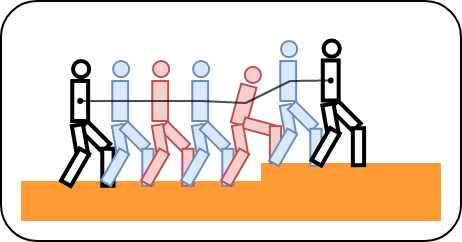
\includegraphics[width=0.7\textwidth, height=5cm]{Figures/Chapter_CPSB/strategies_cp_guide_A.png}
    \caption{Given a guide path, our contact planner generates key configurations in contact along it.}
    \label{fig:cp-sb:strategy_cp-sb}
\end{figure}

% In this chapter, we present our first contact planner which populate the guide path with key configurations in double support contact
%\stn{Il faut faire tres attention ici. Faut commencer par dire que tu as besoin d un contact planner pour valider leas. C est delicat parce que ce st un chapitre entier de ta these qui est pas ta contrib, faut le dire direct}
%In this chapter we present the first contact planner we use in the module P2 of our multi-stage framework for locomotion: an acyclic Sampled-Based Contact Planner (SBCP) \cite{AcyclicCP} for multiped robot locomotion implemented in HPP software \stn{tu peux pas vraiment inventer des noms pour le travail des autres :D. Ou alors tu dis que tu utilises l acronyme pour simplifier} \cite{HPP_software}. We then explain \stn{???}

We have defined in the previous chapter a methodology to learn by reinforcement a local navigation method.
At evaluation time, our method LEAS produces a guide path along which we want to compute a contact sequence.

In a first phase, we used simple termination conditions during the training: the reachability $\tilde{\mathcal{R}^*}$ and the collision-free $\tilde{\mathcal{C}}$ conditions.
Yet those approximated conditions are necessary but not sufficient to guarantee the existence of a feasible contact sequence along the guide.

We now propose to explore the following question: \textit{What is a good guide path to generate a valid contact sequence ?}
For that, we will rely on an existing implementation of a contact planner, which we refer to as the second stage of our framework (P2). 
In this chapter, we use an acyclic Sample-Based Contact Planner \cite{AcyclicCP} for multiped robot locomotion, which for convenience we will refer to as SBCP.
As discussed in Chapter \ref{sec:LEAS}, we want LEAS to achieve two objectives:
\begin{itemize}
    \item Navigating using a local height map of the terrain toward a goal direction subject to some reachability and collision constraints;
    \item Generating guide paths (P1) maximizing the likelihood of finding feasible contact sequences along it with a contact planner (P2).
\end{itemize}
% What is the problem solved
In the context of Motion-before-Contact, LEAS learns to address by reinforcement one of the key limitations of this strategy: the non-guarantee of the feasibility of the guide (P1) by a contact planner (P2).

This chapter is organized as follows:
%section \ref{sub:cp-sb:implementation} we describe how the contact planner is implemented with the offline sampling of limb configurations, the contact generation and their solution to break down the combinatorics.
Section \ref{sub:cp-sb:implementation} is an overview of SBCP and its limitations due to the guide path. While this contact planner is not a contribution to this thesis, it is important to have a strong understanding of its structure and of the success and failure modes.
Section \ref{sub:cp-sb:leas_coupling} shows how to train LEAS with the contact planner as a black-box. 
Section \ref{sub:cp-sb:results} presents a benchmark and analysis of the results obtained by this contact planner with our steering methods.
Finally, section \ref{sub:cp-sb:discussion} discusses about our implementation choices and potential improvements to our work.


\section{Summary of the Sampling Based Contact Planner \label{sub:cp-sb:implementation}}

\subsection{Notations}

The Sample-Based Contact Planner (SBCP) \cite{AcyclicCP} belongs to the motion-before-contact family of contact planners, using a rough robot root trajectory (guide path) to generate the contacts along.
%In this work we do not use the arms of the robot and thus dismiss the multicontact aspect to focus on legged locomotion. \stn{la maniere plus simple de decrire le pb c est de parler de leas et de la validation et de dire naturellement que les scenarios etudies (que tu as deja definis precedemment) sont la marche bipedes}
While it can perform multi-contact locomotion tasks such as standing up or climbing stairs using a handrail, in this work we are interested in biped walking for the scenarios tested in Chapter \ref{sec:LEAS} where we only enable foot contacts with the terrain.
% Notations need to be consistant with part \ref{subsubsec:actions}

\newpage

We use the following syntax:
\begin{itemize}
    \item q$_{base}$ is the robot root configuration in SE$(3)$ (position and orientation);
    \item q$_k$ is the partial robot configuration on limb $k\in\{left\_leg, right\_leg\}$ with 6 degrees of freedom each. The methods allows a more generic multiped setup but we limited our benchmarks to biped cases;
    \item q $= [\mbox{q}_{base},\mbox{q}_{left\_leg},\mbox{q}_{right\_leg}]$ is the robot whole body configuration.
    \item G $ = [\mbox{q}_{base}^0,\mbox{q}_{base}^1,..., \mbox{q}_{base}^{M-1}]$ is the guide path, described as a sequence of M root configurations;
\end{itemize}

%We first explain how we sample the limb configuration of each joint and how we use it for contact creation, then we explain the contact planning process. \stn{pourquoi perdre du temps sur la base de donnees? On s en fout. Tu devrais expliquer le principe et finir en disant que pour gagner du temps on utilise une db. D abord expliquer le concept genereal}

% In this section we present an overview of SBCP, then we expose the feasibility problem with the guide path planner (P1).

\subsection{Overview of the Contact Planner}

%\textcolor{red}{I need to introduce N (samples), Robustness, MAX\_TRIES for repositioning}
\begin{figure}
    \centering
    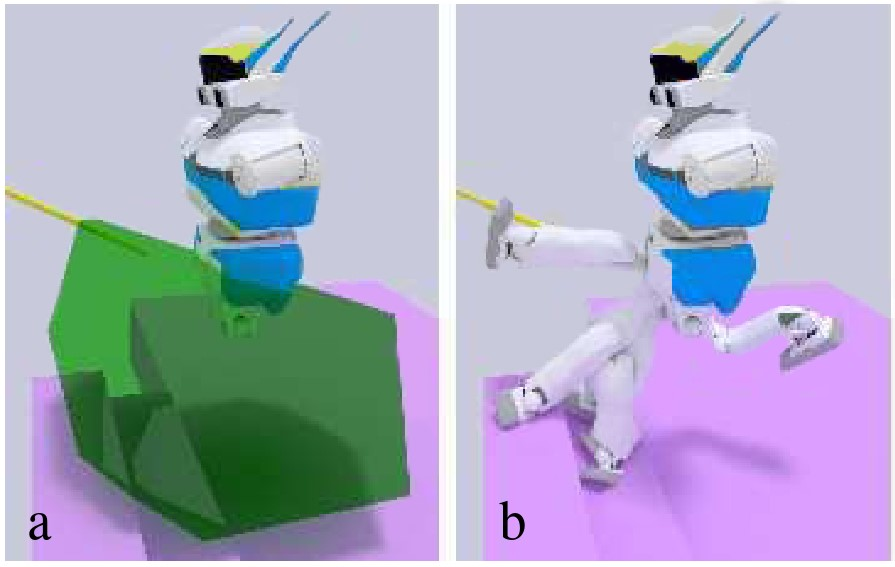
\includegraphics[width=0.6\textwidth, height=5cm]{Figures/Chapter_CPSB/denoised_config_sampled.jpg}
    \caption{Sampling of limb configurations for the right leg of HRP-2 robot with (a) the leg range of motion and (b) some sampled configurations. Source: Tonneau et al. \cite{AcyclicCP}.}
    \label{fig:cp-sb:samples_rom}
\end{figure}

Given an initial whole body configuration $\mbox{q}^0$, the role of SBCP is to populate a guide path in input $G = [\mbox{q}_{base}^0,\mbox{q}_{base}^1,..., \mbox{q}_{base}^{M-1}]$ with a sequence of configurations in contact double support with the terrain and static equilibrium [$\mbox{q}^0$,$\mbox{q}^1$,..., $\mbox{q}^{M'-1}$] following \textbf{exactly} the guide path. 
% Comments steve
%\stn{le guide path il est continu en input, tu le discretises apres non ?} \textcolor{blue}{Non il est toujours discret.} 
%\stn{pourquoi L c est la config et pas q pour tout ? Sinon par convention en general les vecteurs c est minuscule gras, les grandes lettres c est pour les ensembles, ou en gras pour les matrices}

This is done in two steps: first, an offline sampling of limb configurations, second, an online search on these samples for the contacts to perform.

First, an offline database is generated containing configurations q$_k$ for each limb $k$. %to create contacts.
To do so, we randomly sample $N$ configurations for each limb inside their range of motion (Figure \ref{fig:cp-sb:samples_rom}).
This database will be searched at runtime, to select the most suitable limb configuration for a given root according to user-defined heuristics.
% and the measure of the $robustness$ of the equilibrium in the contact forces (More details about the measure of the robustness in \cite{AcyclicCP}). \textcolor{red}{I will use the measure of the robustness later, I don't know if I should explain it more or let it like this.}
We will discuss the heuristics used to search and select contact configurations, in particular the quantification of the robustness of the configuration balance, later in this chapter. %Section \ref{sub:cp-sb:leas_coupling}.

\begin{figure}
    \centering
    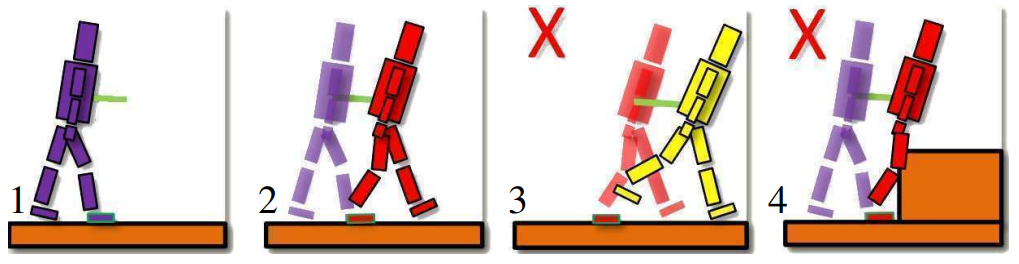
\includegraphics[width=\textwidth]{Figures/Chapter_CPSB/contact_maintain.png}
    \caption{Contacts are maintained on the next root position (green line) if kinematically feasible and without collision (2), they are broken otherwise (2,3). Source: Tonneau et al. \cite{AcyclicCP}.}
    \label{fig:overview_sbcp}
\end{figure}

% Role of the guide, SBCP follows exactly it and try to reach the next position on it.
Starting from a robot configuration $\mbox{q}^i$ in contact whose root is at q$_{base}^i$, the contact planner moves the robot root to the next position on the guide q$_{base}^{i+1}$. To do so, the contact planner performs the following steps (See figure \ref{fig:overview_sbcp}):
\begin{itemize}
    \item Maintain previous contacts: we check kinematically if the contact with the terrain on limb $k$ can be maintained from the next root position q$_{base}^{i+1}$. If not, the contact is broken.
    \item Repositioning: if more than one contact is broken in the previous step, one or more configurations in contact are added at q$_{base}^i$, to ensure that at most one contact is broken between $\mbox{q}^i$ and $\mbox{q}^{i+1}$. 
    %\stn{je pense qu on s en fout de ca} \textcolor{blue}{Il vaut mieux le dire quand meme non ? Surtout par rapport a MAX\_TRIES. Nicolas: c'est ok comme ca.}
    \item Creating contacts: if only one contact is broken, we create a new one with the limb $k$ that has been contact-free the longest. If the contact creation fails, we try to create contact with another free limb or reposition another limb in contact. If no contact can be computed to reach the next root configuration $\mbox{q}^{i+1}$ after a fixed number MAX\_TRIES of trials, SBCP returns the sub-sequence of successful configurations in contact up to $\mbox{q}^i$.
\end{itemize}
In this work, we focus on biped walking and so we perform contact only with the feet of the robot.
%, thus simplifying the algorithm. \stn{on dit pas que c est plus simple, ca simplifie pas l algo }
Obviously, setting a value of MAX\_TRIES $=2$ for the repositioning is sufficient for biped locomotion, where a higher threshold does not improve further its success but increases the computation time.
%Finally the sequence of configurations contains some limb configurations with redundant contacts position, i.e. where the position of the end-effectors are the same.  \stn{ca on s en fout}.
%That is why we only save the "key" configurations where a new contact is created and that we refer as the contact sequence outputed by SBCP. We refer the reader to \cite{AcyclicCP} for further details on the implementation of the contact planner.
% \stn{tu peux faire encore plus synthetique. t as une liste de config, une liste d effecteurs actif, et tu sors une liste de configurations en contact. Ensuite tu listes les raisons pour lesquelles ca va foirer, bonnes ou mauvaises. notamment si le guide est infaisable}
% Description of the complete pipeline RB-PRM (guide + SBCP)
Finally we recall the motion-before-contact strategy of SBCP in Figure \ref{fig:cp-sb:sbcp_explanation} with (a) generation of a guide path from an initial to a goal configuration respecting the reachability constraint $\tilde{\mathcal{R}^*}$ and collision-free $\tilde{\mathcal{C}}$, (b) creation of new contacts to sequentially reach each root configuration along the guide.
% What we said in chapter LEAS

\begin{figure}[h]
    \captionsetup[subfigure]{justification=centering}
    \centering
    \begin{subfigure}[t]{.48\linewidth}
    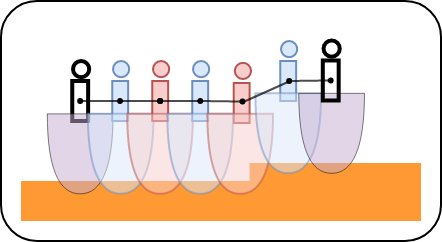
\includegraphics[width=\textwidth, height=4cm]{Figures/Chapter_CPSB/sbcp_explanation_0.png}
    \caption{}
    \end{subfigure}
    \begin{subfigure}[t]{.48\linewidth}
    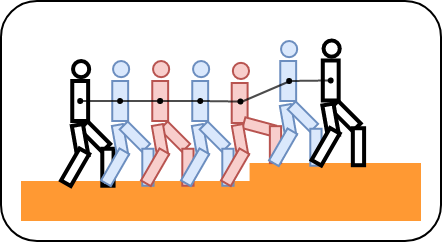
\includegraphics[width=\textwidth, height=4cm]{Figures/Chapter_CPSB/sbcp_explanation_1.png}
    \caption{}
    \end{subfigure}
    \caption{Motion-before-contact strategy with SBCP: (a) generating a valid guide path and (b) computing the key configurations in contact along.}
    \label{fig:cp-sb:sbcp_explanation}
\end{figure}

\subsection{Limitation due to the Guide}

In Chapter \ref{sec:LEAS}, we have shown how LEAS generates guide paths subject to reachability and collision constraints ($\tilde{\mathcal{R}^*}$ and $\tilde{\mathcal{C}}$) for configuration validity. 

We now raise the key problem of the motion-before-contact strategy that is the non-guaranteed feasibility of the guide (P1) by the contact planner (P2).
% which hints us to some limitations of computing a contact sequence with SBCP using such guide paths.
%This limitation is encountered in many scenarios with our contact planner that can fail to compute a contact sequence following exactly a root trajectory.
% Our conclusion
Our experiments will show that the major factor impacting the contact planning success is the guide path in input.
% We do not know what is a "good" guide for SBCP, so it is difficult to approximate the feasibility using some manually designed heuristics. The reachability and collision conditions may not be sufficient
The problem is that we do not know what is a good guide path for this contact planner. 
The reachability and collision conditions introduced for configuration validity are necessary but not sufficient to generate guide paths feasible by this contact planner. 
%\textcolor{red}{Il faut que le sol soit atteignable et que la tronc ne soit pas en collision, sinon on ne peut pas faire de contact.}
As a consequence, it is difficult to define new additional constraints or heuristics to our guide path generator (P1) to better approximate the contact planning feasibility (P2).

Our solution to solve such a feasibility problem is to learn with LEAS how to validate its guide paths with SBCP, which computes the contact sequence along them. In other words, we want LEAS to answer the question: \textit{What is a feasible guide path for this contact planner ?}

%Finally, the resulting solution for the contact planning problem, LEAS plugged to SBCP, should be computationally efficient and present a better success rate than with our previous steering methods RB-Lin and RB-Kino on a wide range of scenarios.


% Problems more in details
%In our experiments, we found many cases where the guide paths even though valid (i.e. ground reachable and no collision along them) lead to a failure with SBCP on our test scenarios, thus motivating our search for a better steering method (P1).
%More specifically, we want to plug SBCP to LEAS to learn by reinforcement how to generate guide paths better fitting this contact planner.


\subsection{Trade-off in the Parameters \label{subsub:cp-sb:tradeoff}}
%\textcolor{blue}{Nicolas: Failure modes of the contact planner}

%We presented the overall concept of SBCP and the problem we are trying to solve in this section.
Before jumping onto our solution with LEAS, we identify two critical parameters whose tuning strongly impacts the success rate and the computation time of the contact planner:
\begin{itemize}
    \item $N$, the number of randomly sampled configurations q$_k$ for each limb $k$;
    \item $\Delta D$, the discretization step on the guide path, corresponding to the average distance between each root configuration q$_{base}^i$ to q$_{base}^{i+1}$ provided as input to the contact planner. 
    %\stn{tel que tu as ecrit les inputs ca arrive déjà discrétise...} \textcolor{blue}{C'est le cas.}
\end{itemize}
The first parameter $N$ is set offline, when initializing the database of limb configurations. The second parameter $\Delta D$ corresponds to the guide path discretization.
A trade-off has to be found on these values to comply with the requirements on the computation time and the success rate of the contact planner.
That is why we provide an analysis of both parameters and explain our choices for this work. The results are presented in Figure \ref{fig:cp-sb:impact_param_tuning}.

\begin{figure}[ht]
    \centering
    \captionsetup[subfigure]{justification=centering}
    \centering
    \begin{subfigure}[t]{.48\linewidth}
    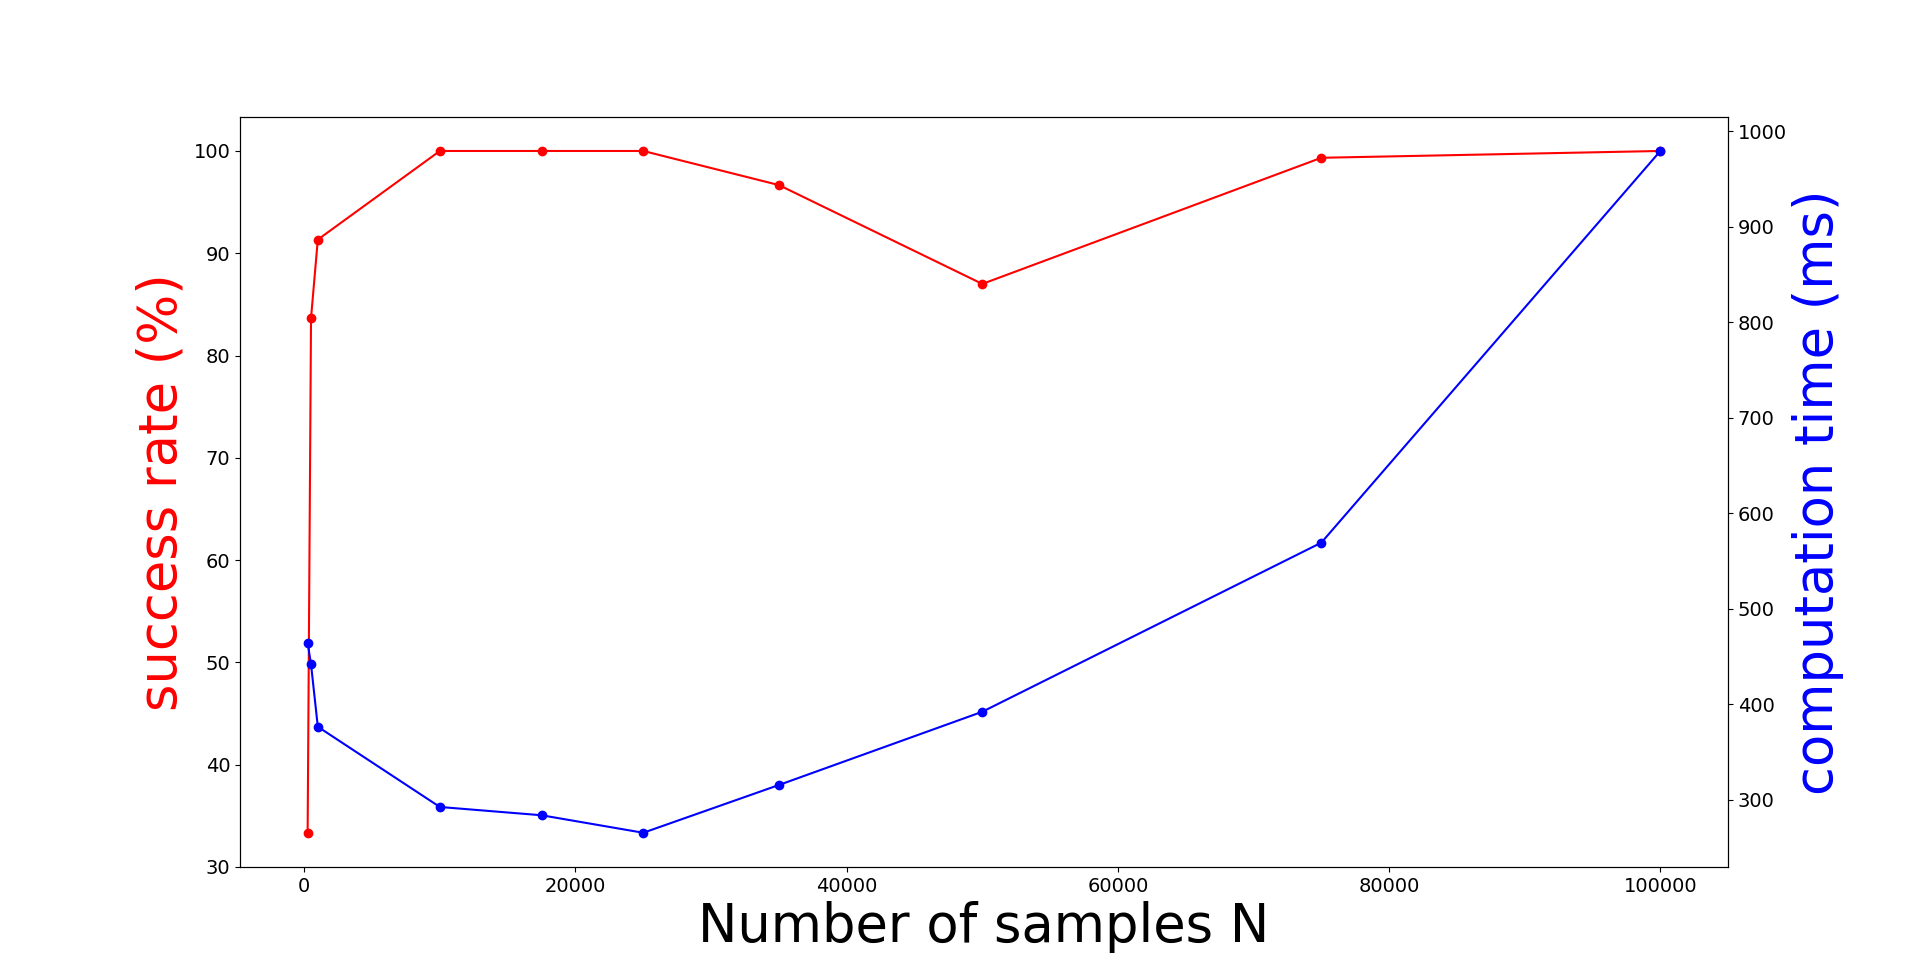
\includegraphics[width=\textwidth, height=4cm,trim={0.5cm 0.5cm 0.5cm 0.5cm},clip]{Figures/Chapter_CPSB/success_time_samples.png}
    \caption{}
    \label{fig:cp-sb:impact_param_tuning:a}
    \end{subfigure}
    \begin{subfigure}[t]{.48\linewidth}
    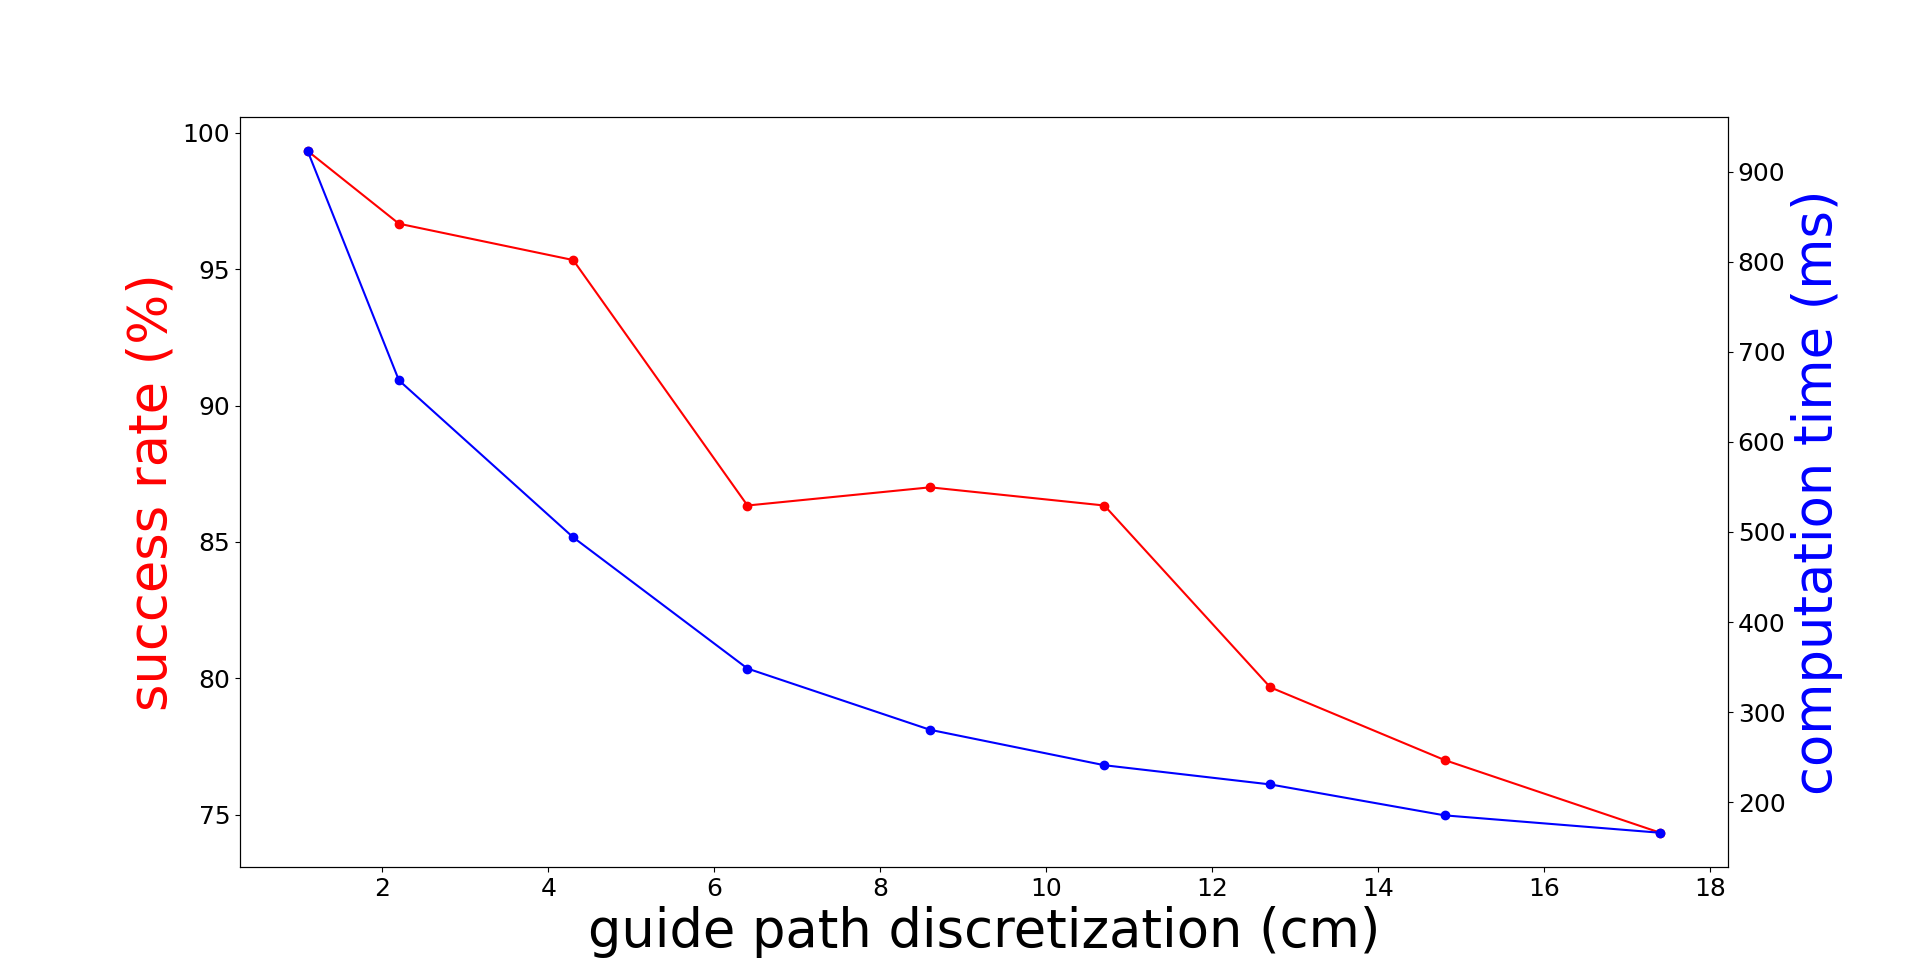
\includegraphics[width=\textwidth, height=4cm,trim={0.5cm 0.5cm 0.5cm 0.5cm},clip]{Figures/Chapter_CPSB/success_time_discretization.png}
    \caption{}
    \label{fig:cp-sb:impact_param_tuning:b}
    \end{subfigure}
    \caption{Analysis of the success rate and computation time of SBCP with a guide path computed by RB-Kino in function of: (a) the number of samples $N$ and (b) the guide path discretization $\Delta D$ (average distance between the root configurations).}
    \label{fig:cp-sb:impact_param_tuning}
\end{figure}

\paragraph{Number of samples.}
The random sampling strategy consists in building a database of available configurations for each limb of the robot that is searched during the contact creation.
The number of samples $N$ is thus critical to provide enough coverage of the robot leg range of motion.
In this test, we measure the impact of the number of samples on the success rate and the computation time for complete successful guide paths only (Figure \ref{fig:cp-sb:impact_param_tuning:a}).
The success of a guide path is defined as the percentage of the successful guide with SBCP. For example, with a guide path of 100 configurations, if the contact planner fails to reach the configuration of index 50 then the success value is $50$\%.
% About the seed : it's complex, actually a seed with 25k samples work perfectly, but not with 50k...
We perform this test on the climbing stairs scenario (see Section \ref{sec:cp-sb:par:stairs}) where we generate some valid guide paths with RB-Kino from 100 uniformly sampled initial positions at the bottom of the stairs oriented toward the goal. 
We then evaluate the results of different sample values $N$ for 3 different seeds, with an average guide path discretization step $\Delta D = 2$cm. 
We will explain the choice of $\Delta D$ later on in this section.

We observe that (red) the success rate rapidly converges to a maximum success rate on this task, and that (blue) the contact planning time increases with the number of samples $N$.
From these results, we can deduce that a number of samples $N=10K$ is sufficient to solve this particular locomotion task.
However, reducing the value of this parameter beyond a certain point increases the computation time, where the contact planner requires contact repositioning to compensate for the lack of sampled configurations leading to a robust solution.
As a result, we found the sweet spot to be $N=25K$ for the stairs and that we keep fixed in our setting across our scenarios. 
It is unsure how this small number of samples copes with more complex terrains like our 5x30 training ground, but we can expect a lower feasibility space with SCBP and where the guide path quality becomes more important.


\paragraph{Guide path discretization.}
The discretization step $\Delta D$ on the guide path corresponds to the average distance between each root configuration q$_{base}^i$ to q$_{base}^{i+1}$. A small $\Delta D$ means a higher number of root configurations on the guide, that results in a higher number of footsteps with SBCP. 
A small value increases its success rate but also its computation time as observed in Figure \ref{fig:cp-sb:impact_param_tuning:b}.
% How is the test done
This test is performed on the same stairs scenario with the steering method RB-Kino. 
RB-Kino generates guide paths continuous in time with non-constant velocities that
we discretize with a fixed timestep. 
We sample some timestep values and measure the corresponding average velocity on the guide, and thus its discretization step $\Delta D$.
We compute 50 trajectories for each measurement and average the results over 3 different seeds and three sample numbers, $N=\{25,50,100\}$K. 

% Comparison with discretization of the guide in acyclic
We compare these results to the original paper \cite{AcyclicCP} using the robot HRP-2 that has a similar maximum step size to the robot Talos we work on. They state that "in most scenarios the torso of HRP-2 moves about 15 cm (for easy scenarios) between two postures, but only 3 cm for the car egress scenario". 
% Results
From our measurements, we see that a small discretization step $\Delta D=2$ cm on the guide increases the success rate of the contact planner. 
Indeed, it is easier for the robot to create a contact to reach a closer root configuration than a distant one.
%However, a small discretization step also comes at the cost of a higher computation time as SBCP generates more configurations in contact along the guide.
% Find a trade-off
The choice of $\Delta D$ is a trade-off between the success rate and the number of steps (and so the computation time). 
One could just set an average discretization $\Delta D=2$ cm that could maximize the success rate in most scenarios. However, this also results in a high contact planning time (over a second) and a hundred footsteps for a trajectory of $3$ to $4$ meters for the climbing stairs task, which is not tolerable.
In this work, we aim for an average discretization $\Delta D=10$ cm resulting in a satisfactory number of steps and computation time, while providing a sufficient success rate on SBCP with our previous steering methods. 
Just as the tuning of the parameter $N$, such a high value of $\Delta D$ lowers the success rate of the guide with SBCP, and so greater emphasizes the quality of the guide (i.e. the positioning of the root configurations relative to the terrain).
On all our steering methods, we further discretize the guide when required to obtain an average $\Delta D=10$ cm and thus provide a fairer comparison with closely matched settings.

\hfill

% Conclusion
% We said all the possibilities in hpp, say the one that is actually chosen in most of their scenario and what could have been nice to work on.
%We presented the general concept behind our sample-based contact planner (P2) computing a contact sequence following exactly the guide in input (P1). We then presented some parameters to analyze the critical part of such contact planning strategy and conclude it to be the input guide path, that is the focus of our research.
We presented the general concept behind our sample-based contact planner (P2) computing a contact sequence following exactly the guide path in input (P1), and our design choice for two critical parameters.
% Modif of nicolas
As we have seen, it is important to design the guide path to have good properties with respect to the contact planner. 
However, these properties are difficult to express explicitly, making it difficult to build heuristics or a more optimal decision process for computing the guide path. 
We then propose to formulate it as a maximization of the success likelihood of the contact planner, building upon LEAS for the learning algorithm. Let's now see the details of this proposition.

% ========================================================================

\section{Implementation Details\label{sub:cp-sb:leas_coupling}}
% Explain the motivation and clearly state what we want to do and hope.
%Our sample-based contact planner presents several limitations due to the separation with the guide path planner P1. We observe on our previous steering methods RB-Lin and RB-Kino plugged to SBCP a drop in the success rate of the contact planning, highlighting the difficulty to design efficient but general enough heuristics that works well on most problems.

Our goal with our steering method LEAS is to overcome the challenges coming from the connection of the guide path planner and the contact planner with a high-level approach.
We want to generate guide paths that are feasible by the contact planner.

% - it implements a stricter constraint to approximate the contact reachable space, further increasing the probability to have more sampled configurations in contact with the terrain.
In the previous chapter, we have shown how LEAS performs in a navigation task with its local terrain-aware capability.
In simple scenarios, LEAS does not heavily rely on path planning algorithms compared to our previous steering methods, resulting in an overall faster generation of guide paths.
%\stn{il faut que tu remplaces tous tes efficient par des termes precis. En quoi elle est mieux que quoi ? sur quelle metrique?}
We now want to improve the feasibility of the generated guide paths by our sample-based contact planner.
% - RL with the SBCP as a black-box, introduce a synergy between P1 and P2 and attempt to alleviate the previously cited limitations intrinsic and extrinsic of SBCP.
We employ the strategy described in the previous chapter with our Master-Workers architecture where the workers validate the trajectories generated by the LEAS agents, by computing the contact sequence along the guides with SBCP used as a black box.
%To do so, we plug SBCP (P2) as a black-box, that computes the contact sequence along the guides generated by LEAS and feedbacks a validation of it during the learning.

\subsection{Parameters of LEAS with Contact Planner}
% - Implementation detail
% - Network
\paragraph{RL policy.}
We employ the same network architecture, states, actions, rewards, and hyperparameters as described in Chapter \ref{sec:LEAS} and set the number of asynchronous workers computing the contacts to 6.
Our method LEAS takes as input a local height map of the terrain and a direction to the goal to locally navigate the terrain. 
States generated by LEAS are subject to the reachability $\tilde{\mathcal{R}^*}$ and collision-free $\tilde{\mathcal{C}}$ conditions, plus a new additional constraint on the whole guide path that is to succeed with the contact planner, that we will explain later on.

% About the CP param
\paragraph{Contact planner parameters.}
We authorize the contact with the limbs $k=$ \{$left\_leg$, $right\_leg$\} to perform a biped locomotion task only, and generate for each limb a number of samples $N=25$K with a fixed seed (empirically selected). Finally, the number of maximum repositioning attempts in the contact planner is set to MAX\_TRIES $=2$, sufficient for our biped locomotion task.

% About the guide / LEAS
% Originally in LEAS
\paragraph{Guide path discretization.}
The discretization of the guide generated by LEAS corresponds to an average of $\Delta D=2$cm between each configuration. 
As seen in the previous section, this value presents on SBCP the best success rate at the cost of a very high computation time, as it generates contact plans with too many contacts (over a hundred steps to walk 3 to 4 meters).
% What we do
That is why we want to aim for an average $\Delta D=10$cm, presenting a suitable trade-off in computation time and success rate with this contact planner.
To do so, we further discretize the guide path before giving it to the contact planner by only keeping 1 out of 5 root configurations on it, to aim for a discretization step of $\Delta D = 2 \times 5 = 10$cm in average (further discussed in section \ref{sub:cp-sb:discussion}).



\subsection{Validation by the Contact Planner}
\begin{figure}[ht]
    \captionsetup[subfigure]{justification=centering}
    \centering
    \begin{subfigure}[t]{.35\linewidth}
    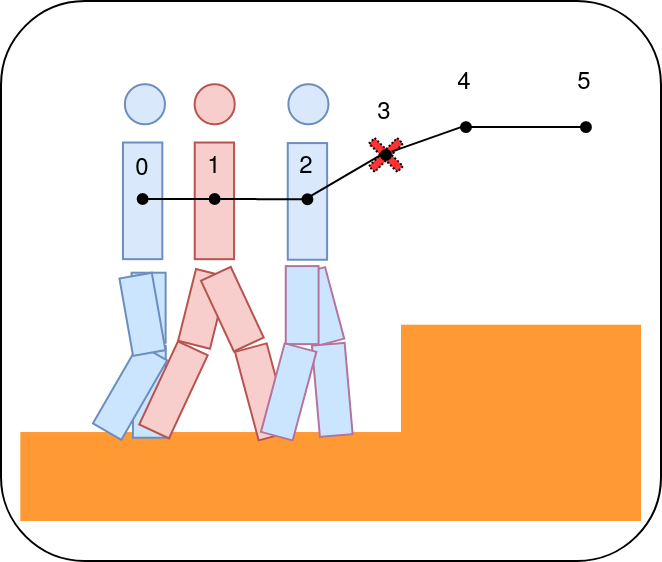
\includegraphics[width=\textwidth, height=4cm]{Figures/Chapter_CPSB/example_fail_planning.png}
    \caption{}
    \end{subfigure}
    \begin{subfigure}[t]{.60\linewidth}
    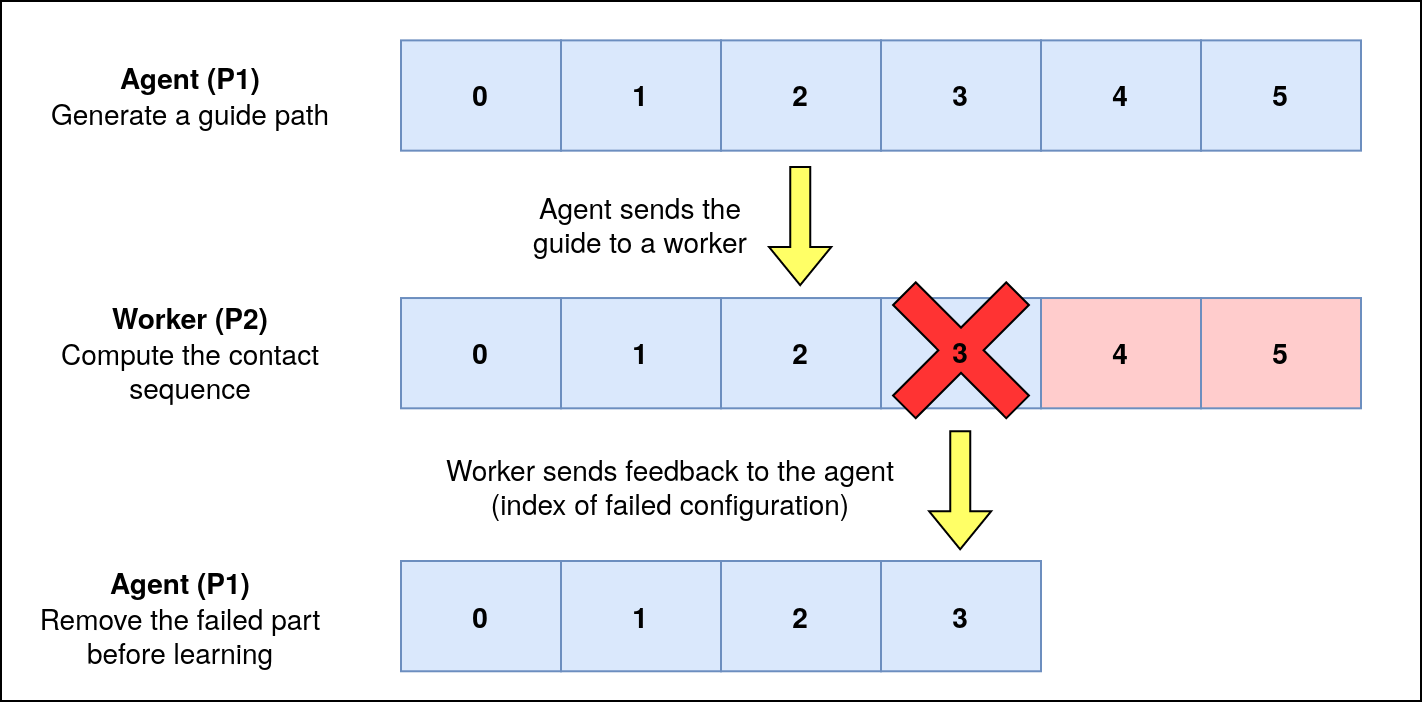
\includegraphics[width=\textwidth, height=4cm]{Figures/Chapter_CPSB/example_fail_planning_diagram.png}
    \caption{}
    \end{subfigure}
    \caption{Generation of a guide path that fails with SBCP: (a) generation of a valid guide path up to configuration 5 and fail of the contact planner at 3, (b) diagram of the learning process from this trajectory.}
    \label{fig:cp-sb:remove_fail_path}
\end{figure}
% What will happen ?
During the learning, the workers perform contact planning with SBCP to validate the trajectories generated by LEAS. Therefore, it learns how to generate feasible guide paths according to the validity conditions $\tilde{\mathcal{R}^*}$ and $\tilde{\mathcal{C}}$, plus the contact planner (P2).
% What is the validation by SBCP
Our contact planner returns the contact sequence along the guide, up to the last successful root configuration q$_{base}^i$.
The index of this configuration is retrieved and sent back to the master that prunes the section of the guide path that failed as depicted in Figure \ref{fig:cp-sb:remove_fail_path}.
% - to learn how to improve the CP-SB success rate => How do we do ? Propagation of the result of CP-SB on the trajectory generated by LEAS.
LEAS has to find a trade-off between learning the navigation task presented in Chapter \ref{sec:LEAS} and succeeding in the contact planning.

\subsection{Training}
\begin{figure}[t]
    \centering
    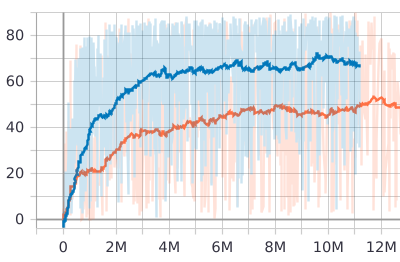
\includegraphics[width=0.6\textwidth]{Figures/Chapter_CPSB/learning_curve_p1_p2.png}
    \caption{Learning curves of (blue) LEAS-P1 trained without contact planner and (red) LEAS-P2 trained with guide validation by SBCP.}
    \label{fig:cp-sb:learning_curves_p1_p2}
\end{figure}
We train LEAS with SBCP on our training terrain presented in the previous chapter.
The model is evaluated after 12 million steps corresponding to 8 hours of training on a PC with an Intel Core i7-8700 (12 cores, 3.20Ghz, 16GB ram). 
Learning curves of LEAS without a contact planner, referred to as LEAS-P1 (Chapter \ref{sec:LEAS}), and LEAS with the contact planner, LEAS-P2, are shown in Figure \ref{fig:cp-sb:learning_curves_p1_p2} (the maximum reward is equal to 100 for trajectories in a straight line at $v_{desired}$). 
The P2 validation increases its probability to meet a terminal condition (i.e. failing the contact planning) and forces LEAS to adapt its behavior to succeed with the contact planner, hence resulting in a lower average reward per episode.

\section{Results\label{sub:cp-sb:results}}

%\paragraph{Evaluation methodology}
For all our tests, we uniformly sample some initial configurations on a flat area and set a fixed goal configuration on the other side of the obstacle to cross, corresponding to trajectories of 3 to 4 meters long in average.
Each steering method has to generate guide paths with valid configurations ($\tilde{\mathcal{R}^*}$ and $\tilde{\mathcal{C}}$) up to the target and compute a contact sequence along it with SBCP.
The success rate presented in the results corresponds to the percentage of valid guide paths reaching the goal and being successful with SBCP.
% Tuning of discretization step
We tune the discretization timestep of RB-Kino and RB-Lin such that the discretization step along the guide is on average equal to $\Delta D=10$cm, just as LEAS.
% Comments
%\stn{comment t usais que c est "fair". Es tu certain qu un pas discret est tjs synonyme de meilleur succes? }

We compare the method proposed in this chapter (LEAS-P2), with the method proposed in the previous chapter (LEAS-P1) and the two model-based steering methods used as benchmarks, RB-Lin and RB-Kino. We evaluate them on scenarios we know, from experience, to be challenging for contact planners. For each scenario, we analyze the changes in the guide path generation, hinting us about our contact planner capability relative to the guide.

\subsection{Scenario A: Rotation\label{subsub:sbcp:rotation}}
Given initial and target configurations, we uniformly sample some initial robot orientations and set some fixed velocity values to evaluate the success of all steering methods with the contact planner. The orientation value corresponds to the angle between the target direction and the root orientation. 
We evaluate the success rate of each steering method that has to rotate and move the robot to the goal. 
This scenario simulates a problem that some heuristic methods cannot solve well. While these methods could be specifically patched to counteract it, it is interesting to understand these behaviors.

In this experiment, all steering methods succeed in generating a valid guide path, reachable and without collision, up to the target but present different results as seen in Table \ref{tab:cp-sb:rotation_success} and Figure \ref{fig:cp-sb:rotation_scenario}. 

\begin{table}[ht]
\centering
\caption{Scenario A: success rate for different orientations on flat ground.\label{tab:SBCP:ground_ori}}
\begin{tabular}{ |c|c|c|c|c| }
    \hline
    \makecell{Parameters} & \makecell{RB-Lin} & RB-Kino & LEAS-P1 & LEAS-P2\\
    \hline
    $0^{\circ}$ to $30^{\circ}$ &  & & & \\
    $||v||$ = 0 & 100\% & 100\% & 100\% & 100\% \\
    $||v||$ = 0.04 & x & 100\% & 100\% & 100\% \\
    $||v||$ = 0.07 & x & 100\% & 100\% & 100\% \\
    \hline
    $60^{\circ}$ to $120^{\circ}$ &  & & & \\
    $||v||$ = 0 & 100\% & 61 \% & 75\% & 100\% \\
    $||v||$ = 0.04 & x & 100\% & 84\% & 100\% \\
    $||v||$ = 0.07 & x & 100\% & 89\% & 100\% \\
    \hline
    $150^{\circ}$ to $180^{\circ}$ &  & & & \\
    $||v||$ = 0 & 100 \% & 0 \% & 22 \% &  100\% \\
    $||v||$ = 0.04 & x & 0 \% & 35 \% & 100\% \\
    $||v||$ = 0.07 & x & 43 \% & 42 \% & 100\% \\
    \hline
\end{tabular}
\label{tab:cp-sb:rotation_success}
\end{table}
\begin{figure}[ht]
    \captionsetup[subfigure]{justification=centering}
    \centering
    \begin{subfigure}[t]{0.49\linewidth}
    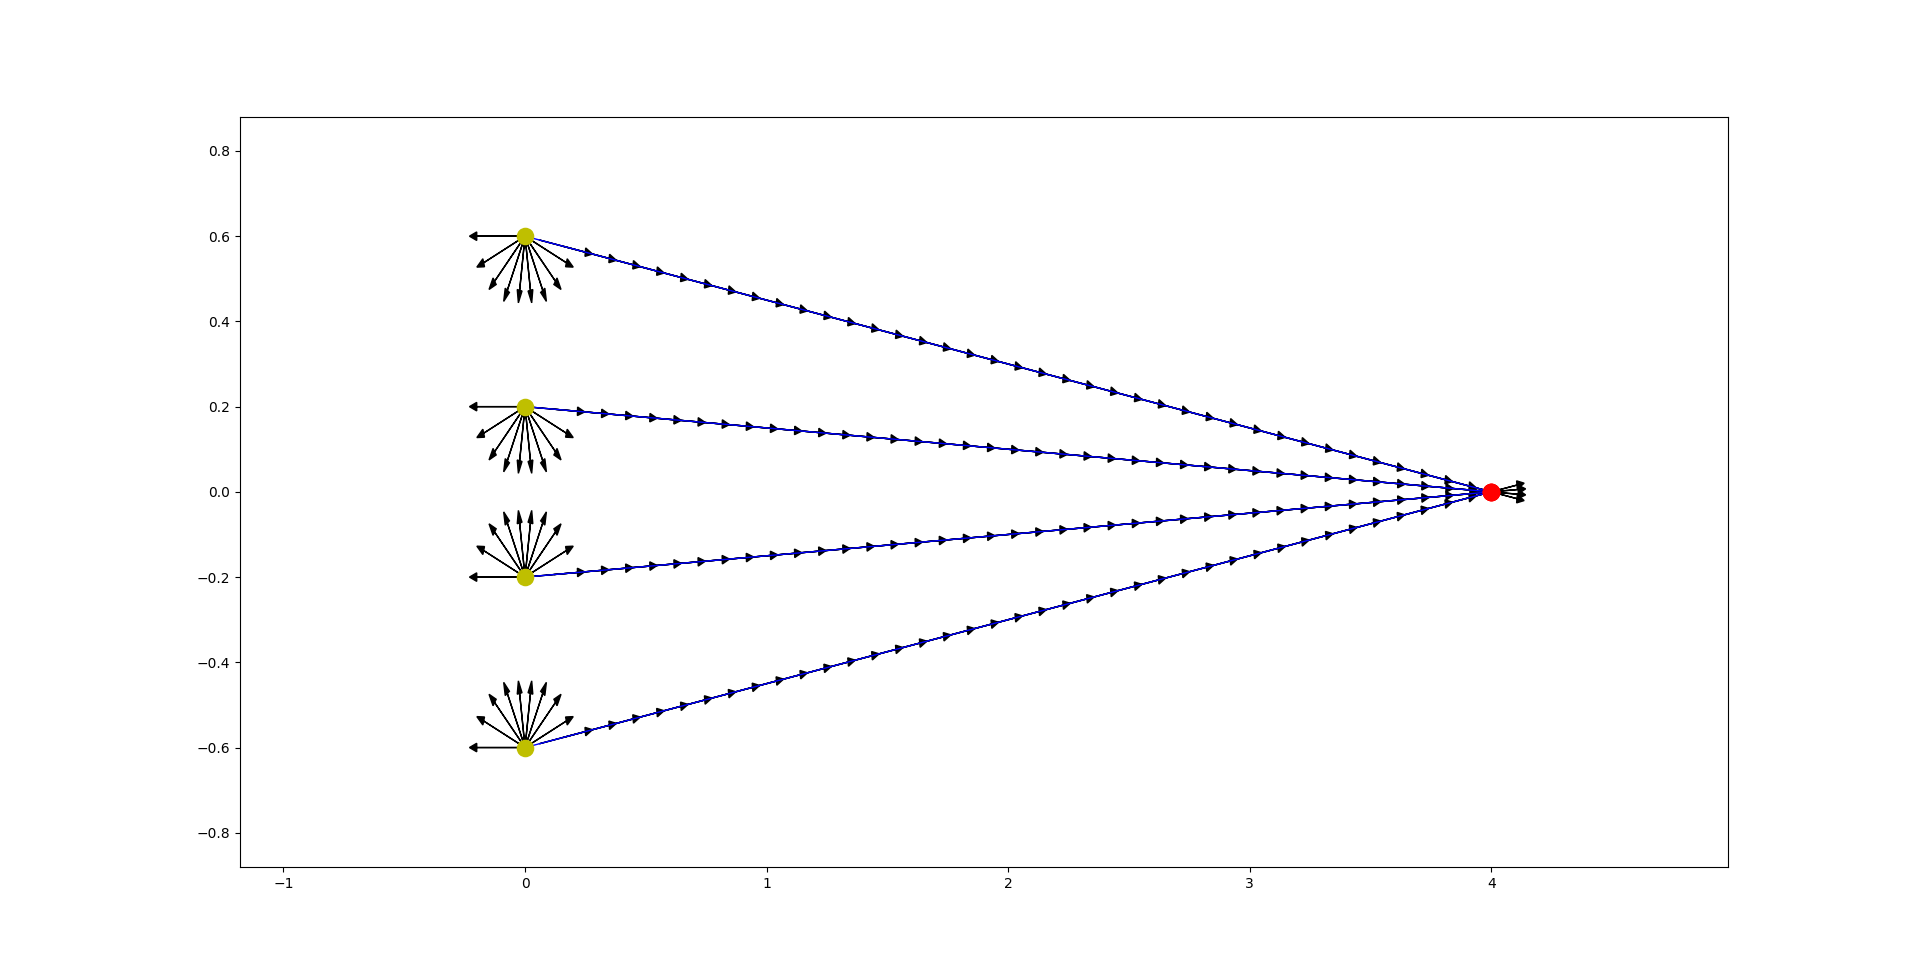
\includegraphics[width=\textwidth]{Figures/Chapter_CPSB/rotation_lin_180_v04.png}
    \caption{RB-Lin}
    \end{subfigure}
    \begin{subfigure}[t]{0.49\linewidth}
    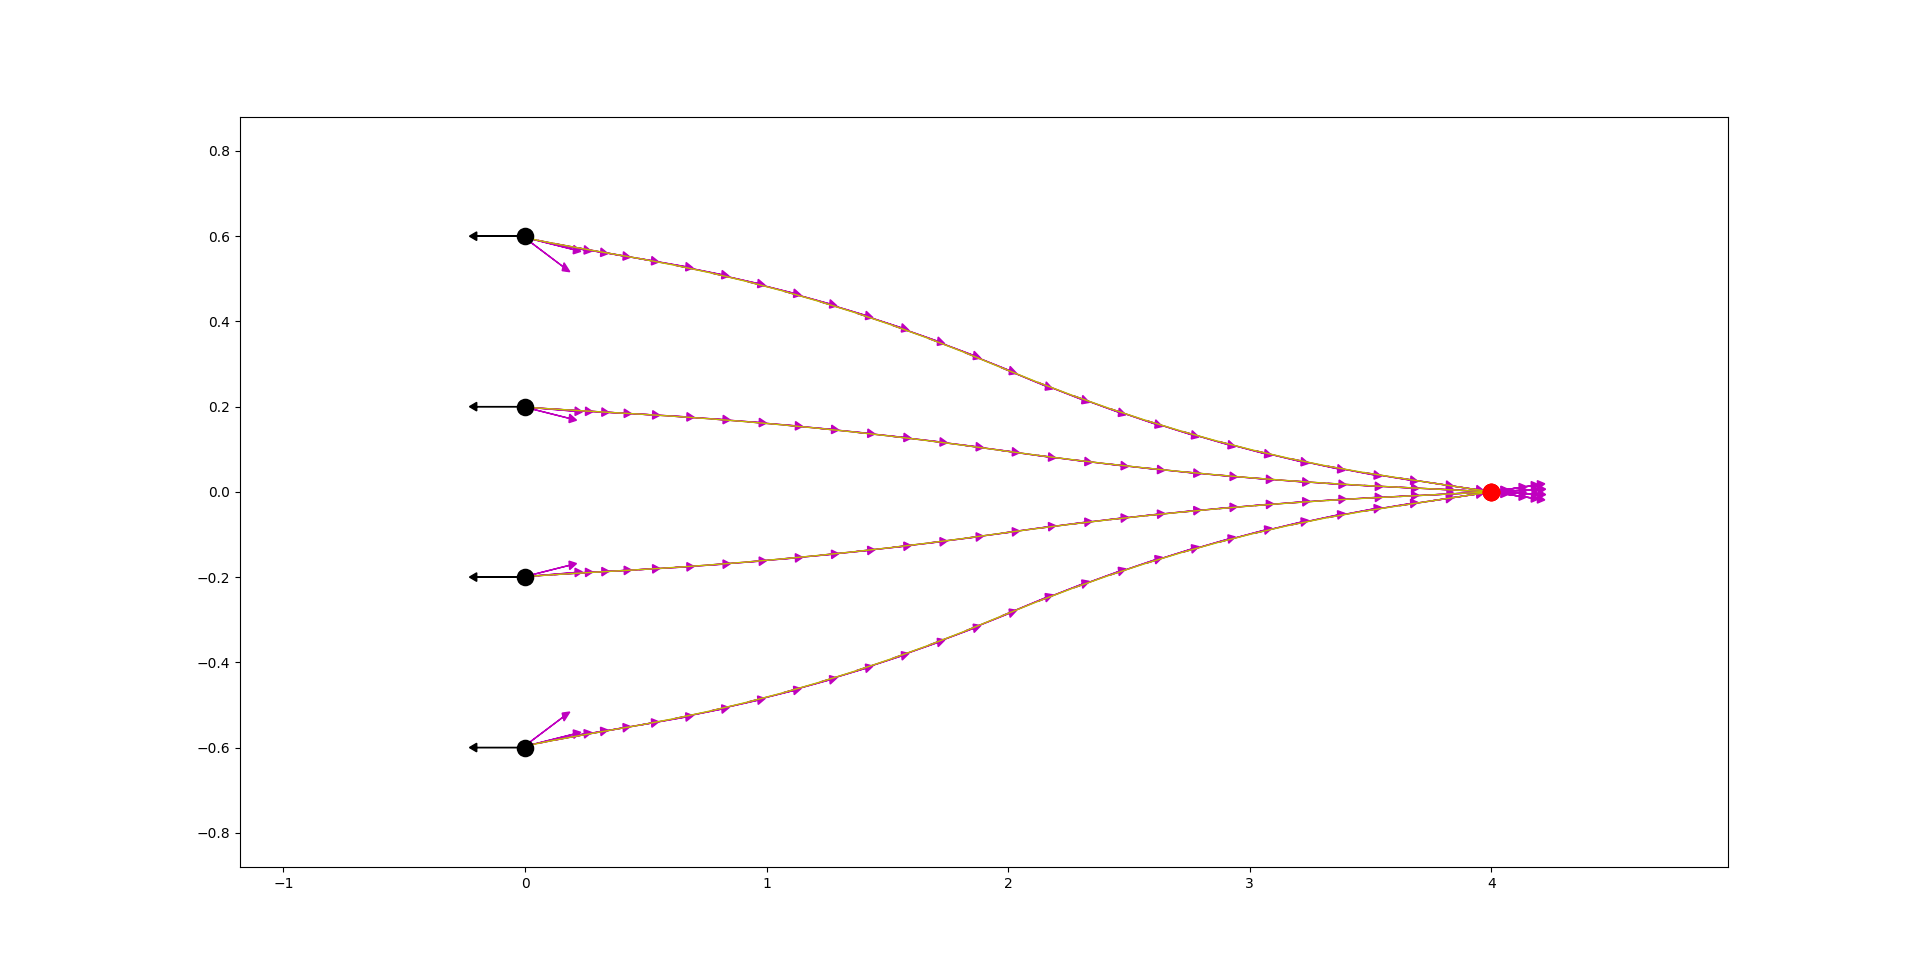
\includegraphics[width=\textwidth]{Figures/Chapter_CPSB/rotation_kino_180_v04.png}
    \caption{RB-Kino}
    \end{subfigure}
    \begin{subfigure}[t]{0.49\linewidth}
    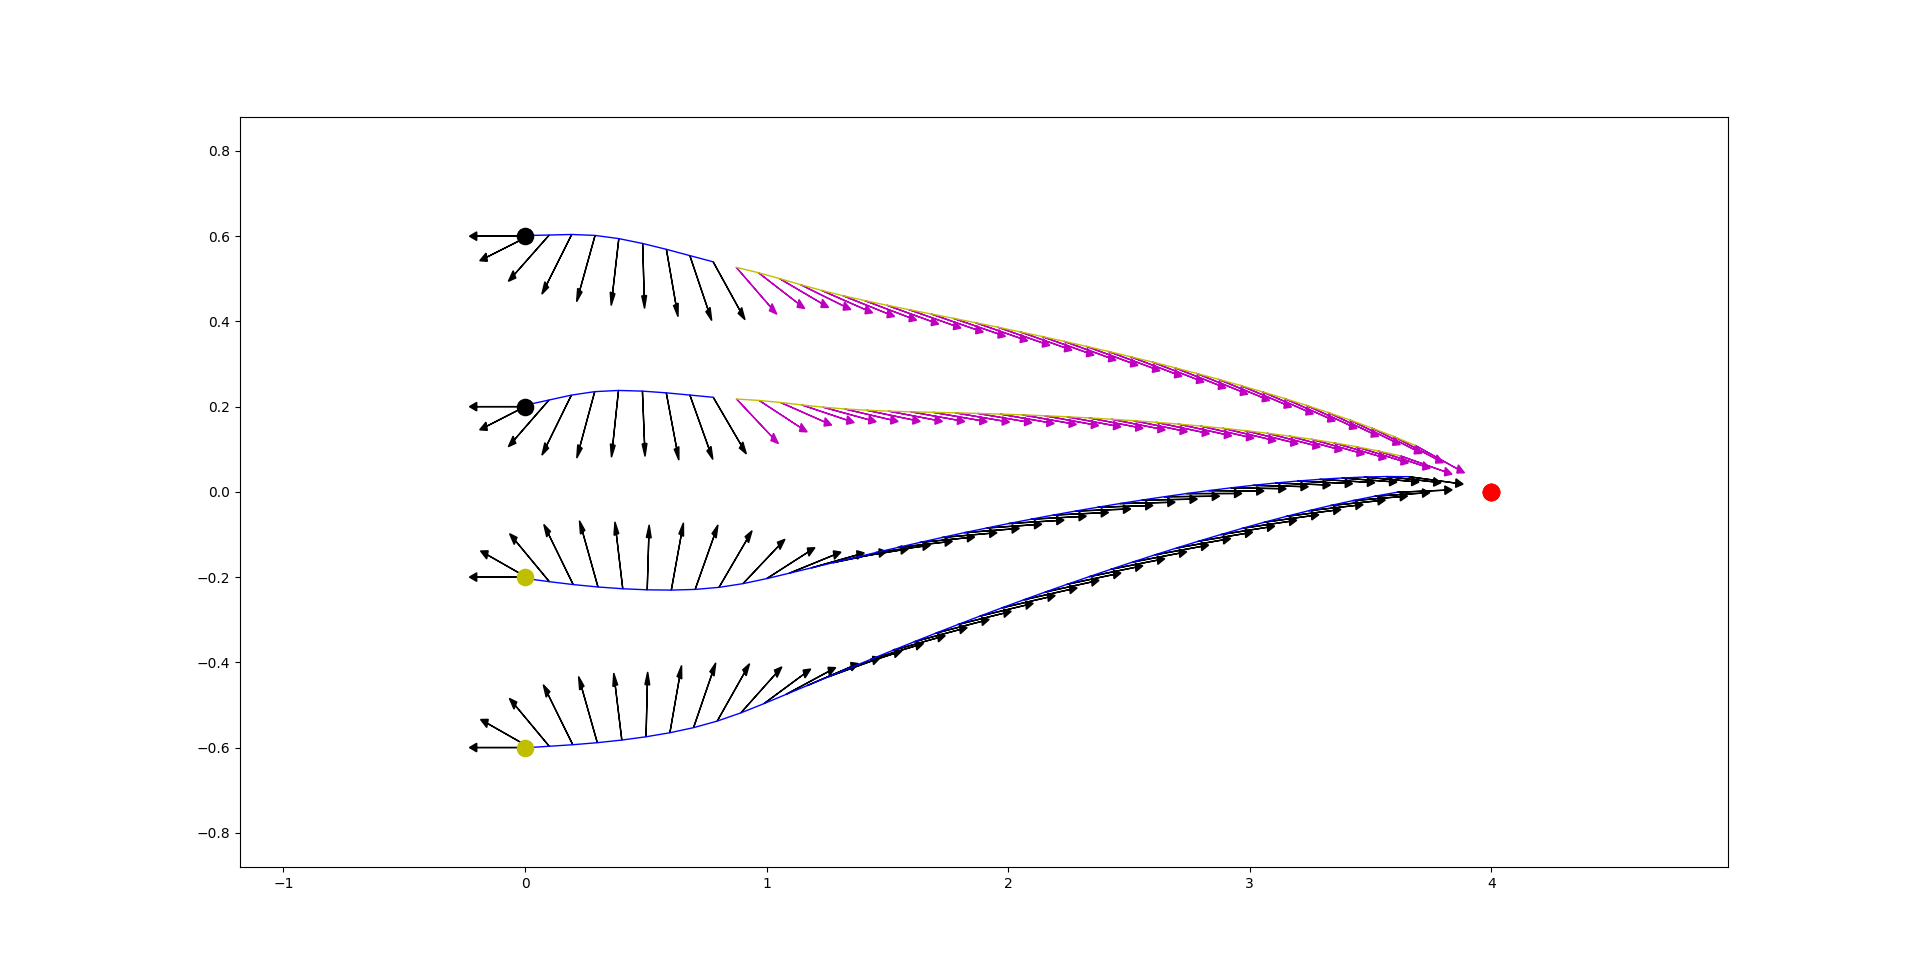
\includegraphics[width=\textwidth]{Figures/Chapter_CPSB/rotation_p1_180_v04.png}
    \caption{LEAS-P1}
    \label{fig:cp-sb:rotation_scenario:leas_p1}
    \end{subfigure}
    \begin{subfigure}[t]{0.49\linewidth}
    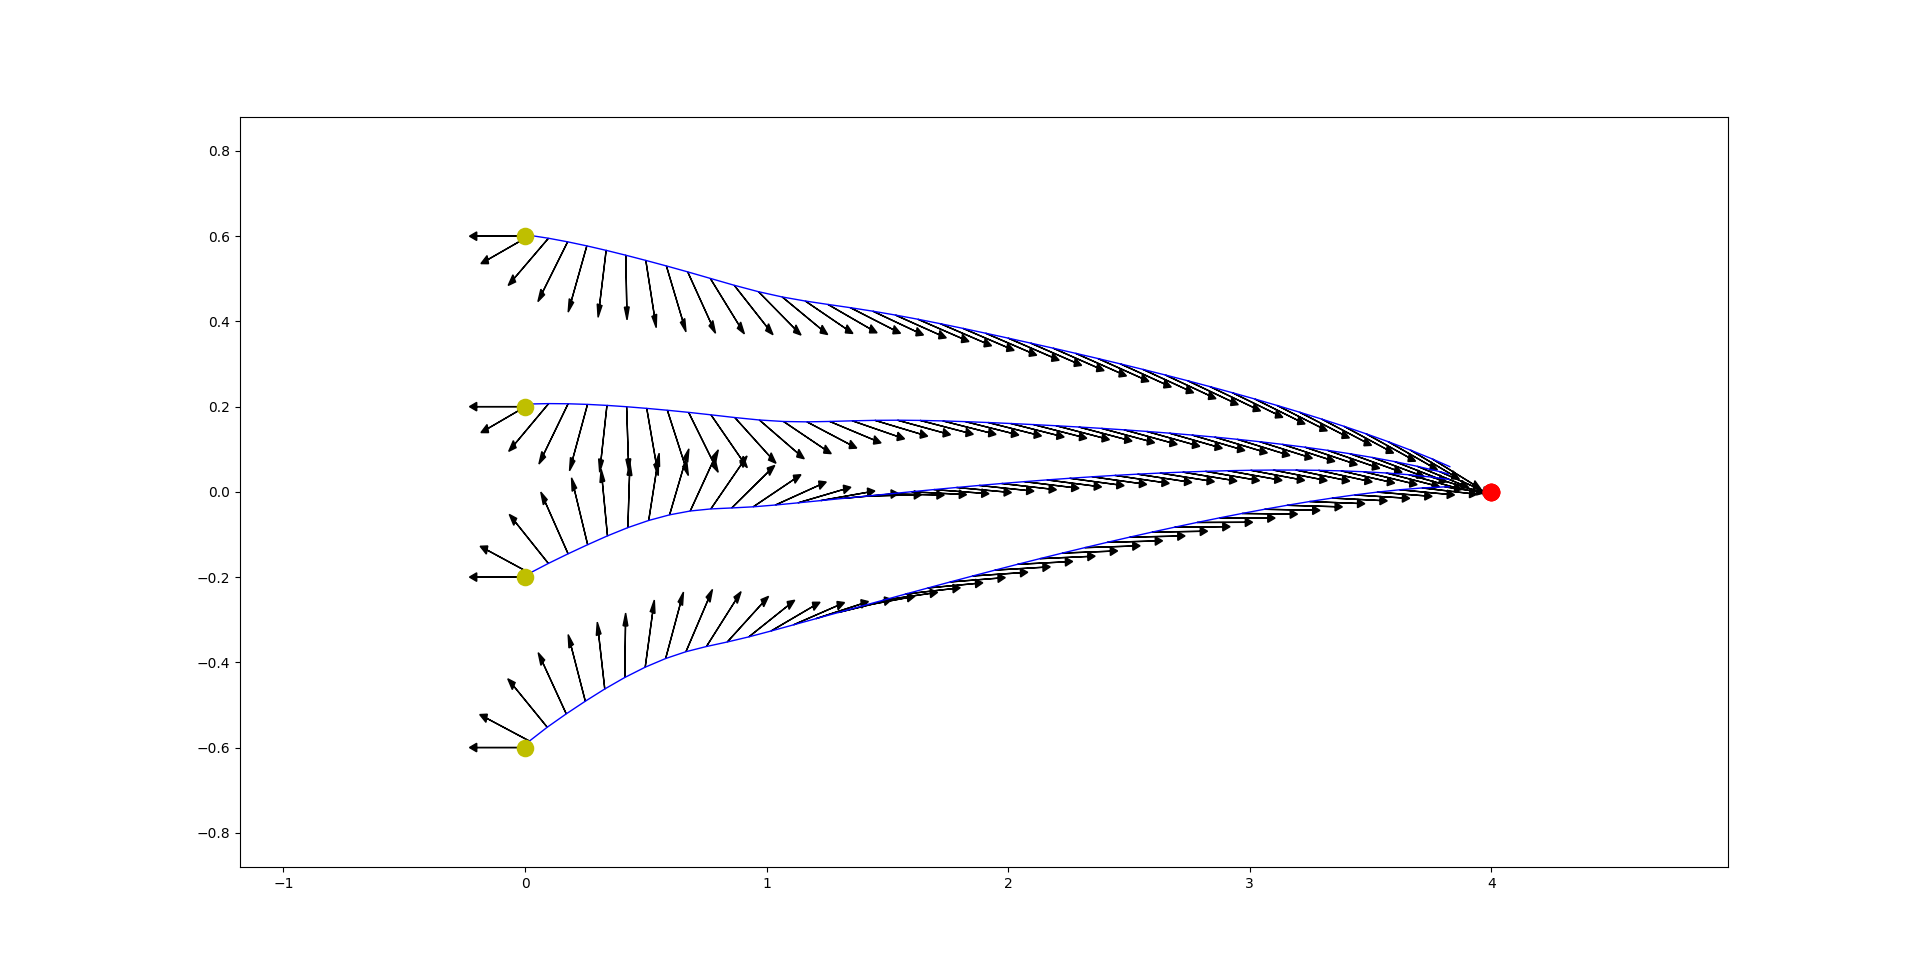
\includegraphics[width=\textwidth]{Figures/Chapter_CPSB/rotation_p2_180_v04.png}
    \caption{LEAS-P2}
    \label{fig:cp-sb:rotation_scenario:leas_p2}
    \end{subfigure}
    \caption{Scenario A, Trajectories for initial configurations at $180^{\circ}$ and $||v||=0.04$ m/s with (blue) the successful and (yellow) the failed part of the guide, and (black arrow) the robot root orientation.}
    \label{fig:cp-sb:rotation_scenario}
\end{figure}
\begin{figure}[ht]
    \captionsetup[subfigure]{justification=centering}
    \centering
    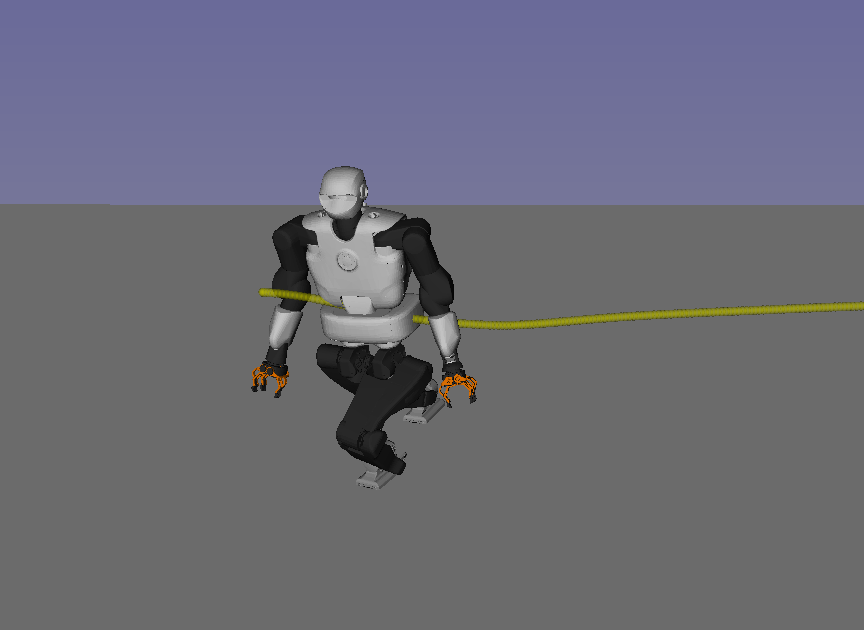
\includegraphics[trim={2cm 2cm 4cm 2cm}, clip,width=0.32\textwidth]{Figures/Chapter_CPSB/rotation_seq/rot2.png}
    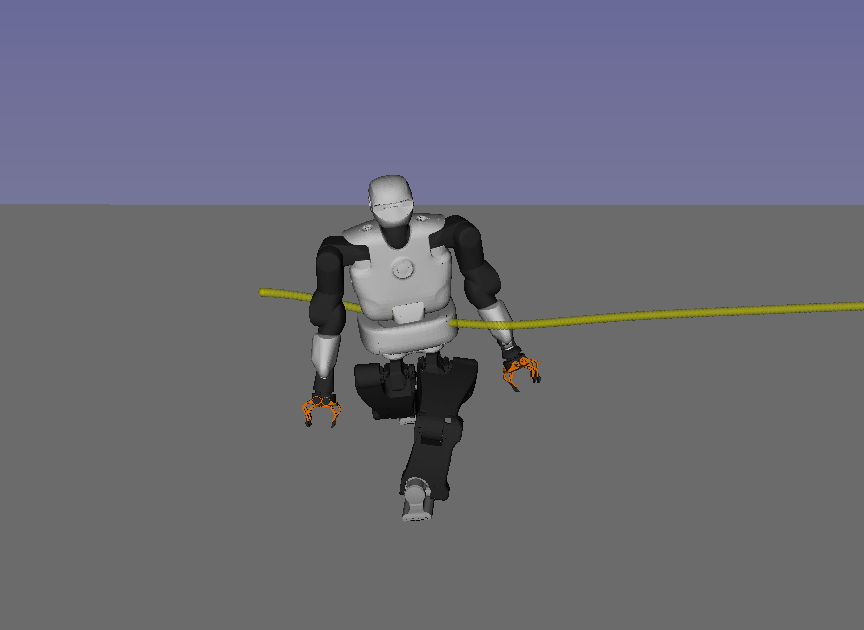
\includegraphics[trim={2cm 2cm 4cm 2cm}, clip,width=0.32\textwidth]{Figures/Chapter_CPSB/rotation_seq/rot3.png}
    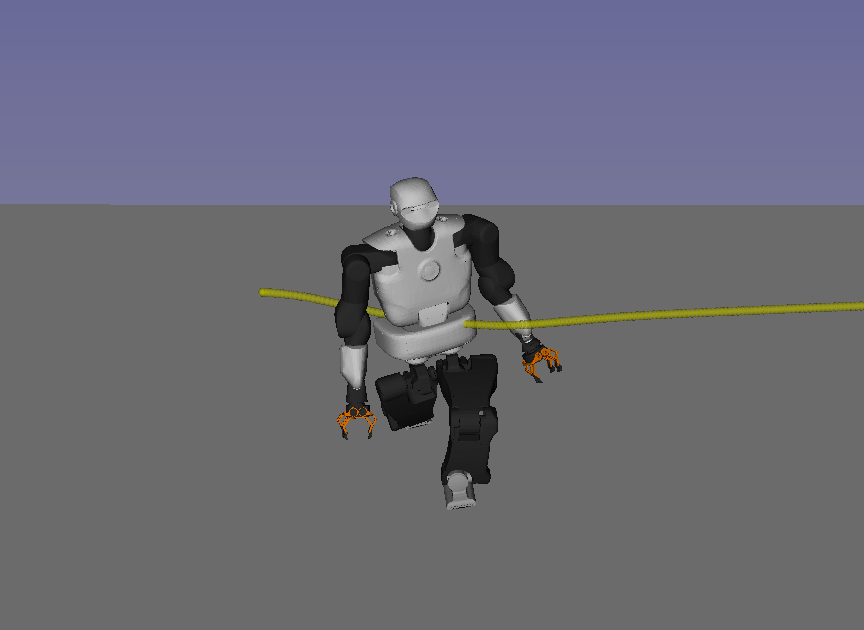
\includegraphics[trim={2cm 2cm 4cm 2cm}, clip,width=0.32\textwidth]{Figures/Chapter_CPSB/rotation_seq/rot4.png}
    \caption{Scenario A: Sequence of configurations where LEAS-P1 fails the rotation along the guide.}
    \label{fig:cp-sb:rotation_leas_p1_fail}
\end{figure}

% RB-Lin results => Work all the time with $\omega_{max}$, it's like a sanity test.
RB-Lin rotates at a fixed angular velocity $\omega_{max}=\frac{\pi}{9}=20$ deg/s which is equal for $T=0.2$ s to a maximum rotation of $\omega_{max} \times T \times 5 = 20^{\circ}$ between each configurations on the guide (keeping 1 out 5 guide configurations).
As expected, the results show that for any initial orientation, rotating the robot with a step angle of $20^{\circ}$ before moving it to the goal generates feasible guide paths by the contact planner. 
RB-Lin shows that a rotation toward the goal, with a step angle $20^{\circ}$ between the guide path configurations, can safely be performed before moving the robot. 
In our tests, all step angles in the range $]0,90]$ degrees were successful, but in practice, a step angle of $45^{\circ}$ may be the maximum feasible by the Talos robot in reality.

RB-Kino succeeds for all orientations in $[0,120]$ degrees. 
However, we can see the limitation of RB-Kino when starting with a (near) null velocity as discussed in the previous chapter, and as a result, fails the contact planning as such high rotation is not kinematically feasible. 
We recall that in practice we adopt the same strategy that RB-Lin by rotating the robot first before using RB-Kino, and thus we always avoid such cases.
% Comments steve
%\stn{on avait dit qu on en parlait pas ? c est un bug facilement contournable, tu devrais mettre 100 la} 
%\textcolor{blue}{Dans ce cas la, ce test sur la rotation ne sert a rien non ? Vu qu'on va toujours tourner le robot vers l'objectif avant de le faire bouger et on aura 100\% de succes partout. J'explique bien apres qu'en general avec RB-Kino on ne va jamais se retrouver dans ce cas la. Nicolas: Il a barré cette discussion donc je suppose que ca veut dire ok.}

Then we compare LEAS-P1 and LEAS-P2 that have been trained with and without feedback from the contact planner respectively.
% What these two agents share in common and do not.
LEAS-P1 is subject to two major rewards motivating its behavior: $R_{ori}$, encouraging him to be oriented to the target and $R_{dir}$ to move toward it at $v_{desired}$. 
As a result, LEAS-P1 balances these two rewards by moving and rotating at the same time. 
Additionally, LEAS-P2 is subject to another constraint that is to succeed with the contact planner (P2).

% Results of LEAS-P1
The results show that LEAS-P1 works for all initial orientations in $[0,30]$ degrees but may fail for initial orientations superior to $60^{\circ}$.
%It is interesting to note that LEAS has its angular velocity $\omega < \omega_{max}$ but fails some rotations compared to RB-Lin. 
Indeed, rotating while moving toward the target is more difficult and requires adapting simultaneously the robot velocity and angular velocity.
Finally, as the initial velocity increases, we can note that so does the success rate with LEAS-P1 and RB-Kino.

% Results of LEAS-P2
In contrast, LEAS-P2 learns how to rotate and succeeds in every rotation scenarios, thus showing the benefit of our solution.
% Analyze how LEAS-P2 rotates better than LEAS-P1 => Visually + how it sacrifices the reward (no sacrifice for this scenario) ?
%However it is difficult to evaluate why LEAS-P2 presents a better success rate than LEAS-P1 (Figure \ref{fig:cp-sb:rotation_scenario}). 
Empirically, we noticed that LEAS-P2 tends to move in the direction of its orientation to help the rotation task (Figure \ref{fig:cp-sb:rotation_scenario:leas_p2}), whereas backward translations with LEAS-P1 could result in failure due to heuristics defined in the contact planner (Figure \ref{fig:cp-sb:rotation_scenario:leas_p1}).
That is why some guide paths generated by LEAS-P1 leads to some configurations that do not permit further movement (Figure \ref{fig:cp-sb:rotation_leas_p1_fail}). 
In contrast, LEAS-P2 automatically discovers how to generate guide paths avoiding the selection of such configurations from the samples.


\subsection{Scenarios B: Obstacle Avoidance}
% Use the hole and bridge from 1x11.
% Hole and bridge are quite similar because when the SM succeeds, it often passes very close to the edge and should avoid it to succeed SBCP.
\begin{figure}[t]
    \captionsetup[subfigure]{justification=centering}
    \centering
    \begin{subfigure}[t]{0.48\linewidth}
        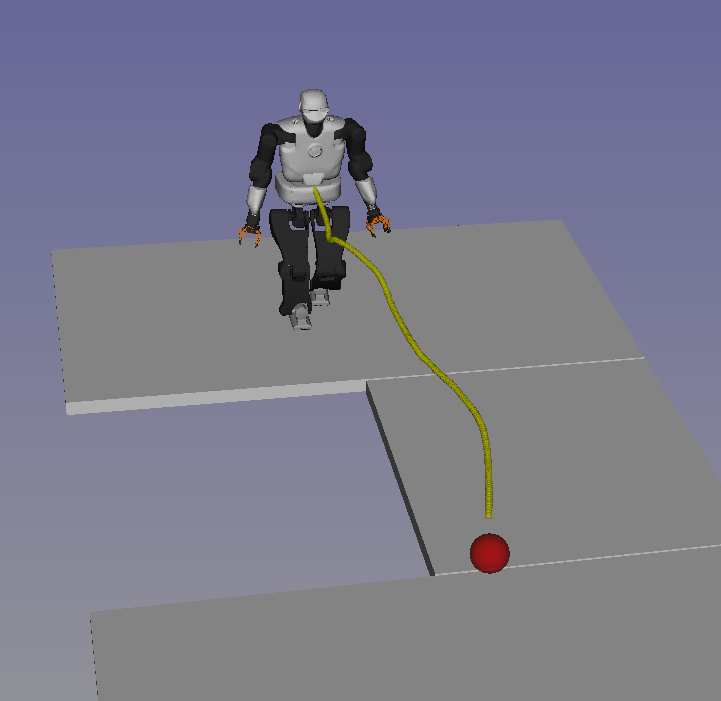
\includegraphics[width=\textwidth, height=6cm]{Figures/Chapter_CPSB/hole_scenario.png}
    \end{subfigure}
    \begin{subfigure}[t]{0.48\linewidth}
        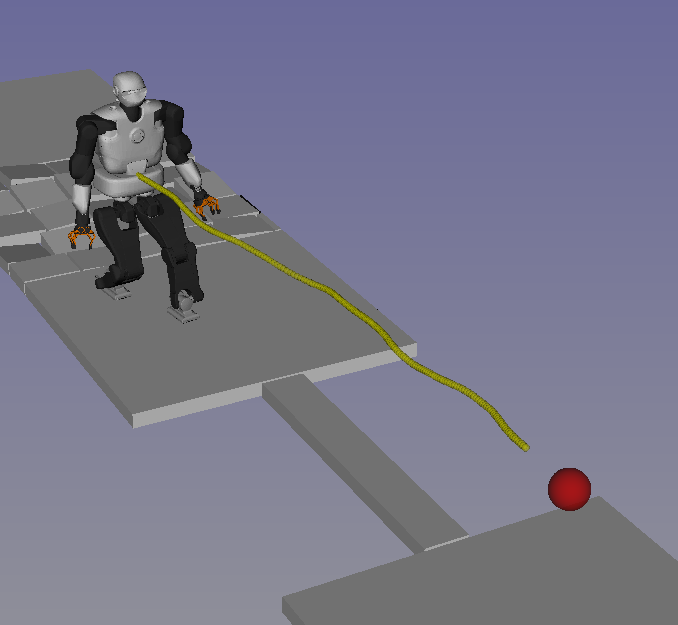
\includegraphics[width=\textwidth, height=6cm]{Figures/Chapter_CPSB/bridge_scenario.png}
    \end{subfigure}
    \caption{Scenario B1: The steering method has to generate a valid guide path (yellow) up to the goal (red), then compute a contact sequence along it with SBCP.}
    \label{fig:cp-sb:scenarios_hole_bridge}
\end{figure}

\begin{table}[h]
\centering
\caption{Scenario B1: Comparison on the success rate and robustness.}
\begin{tabular}{ |c|c|c|c|c|c| }
    \hline
    Parameters & Terrains & RB-Lin & RB-Kino & LEAS-P1 & LEAS-P2\\
    \hline \hline
    \multirow{3}{*}{SR} & Hole & 82\% & 74\% & 100\% & 100\% \\
    \cline{2-6}
                        & Bridge & 86\% & 78\% & 96\% & 100\% \\
    \hline \hline
    \multirow{3}{*}{Robustness} & Hole & 21.7 & 20.9 & 32.2 & 33.3 \\
    \cline{2-6}
                        & Bridge & 20.84 & 25.8 & 24.36 & 27.3 \\
    \hline
\end{tabular}
\label{tab:cp-sb:hole_bridge}
\end{table}

\begin{figure}[ht]
    \captionsetup[subfigure]{justification=centering}
    \centering
    \begin{subfigure}[t]{0.4\linewidth}
        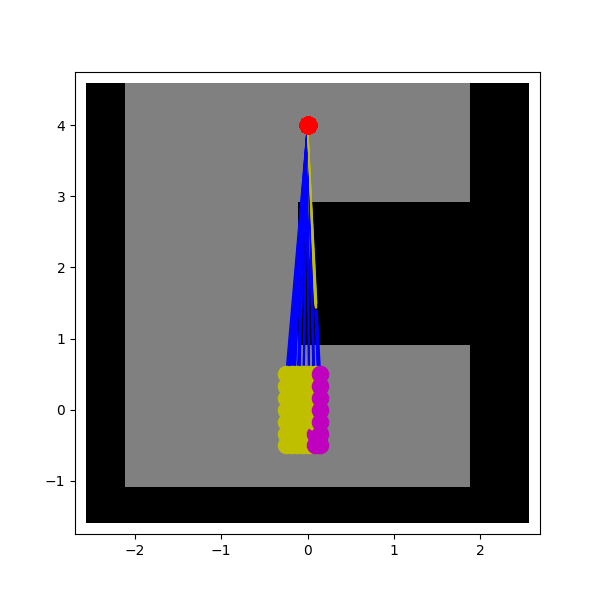
\includegraphics[width=\textwidth, height=3.5cm, trim={0cm 1cm 0cm 1cm},clip]{Figures/Chapter_CPSB/hole_Lin.png}
        \caption{RB-Lin}
    \end{subfigure}
    \begin{subfigure}[t]{0.4\linewidth}
        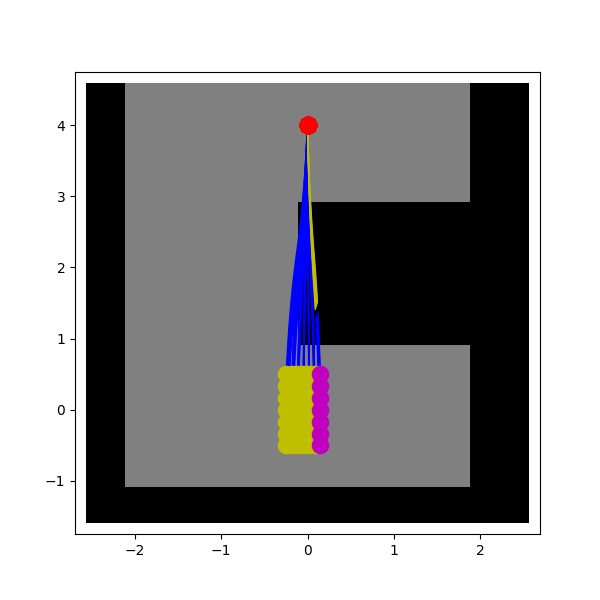
\includegraphics[width=\textwidth, height=3.5cm, trim={0cm 1cm 0cm 1cm},clip]{Figures/Chapter_CPSB/hole_Kino.png}
        \caption{RB-Kino}
    \end{subfigure}
    \begin{subfigure}[t]{0.4\linewidth}
        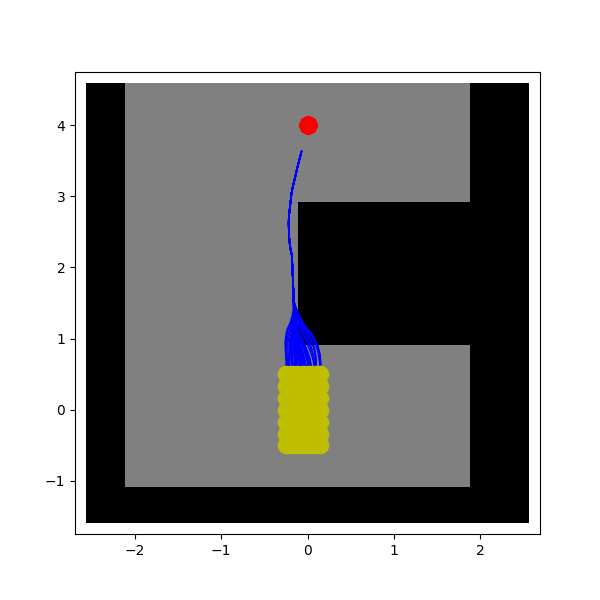
\includegraphics[width=\textwidth, height=3.5cm, trim={0cm 1cm 0cm 1cm},clip]{Figures/Chapter_CPSB/hole_LEAS-P1.png}
        \caption{LEAS-P1}
    \end{subfigure}
    \begin{subfigure}[t]{0.4\linewidth}
        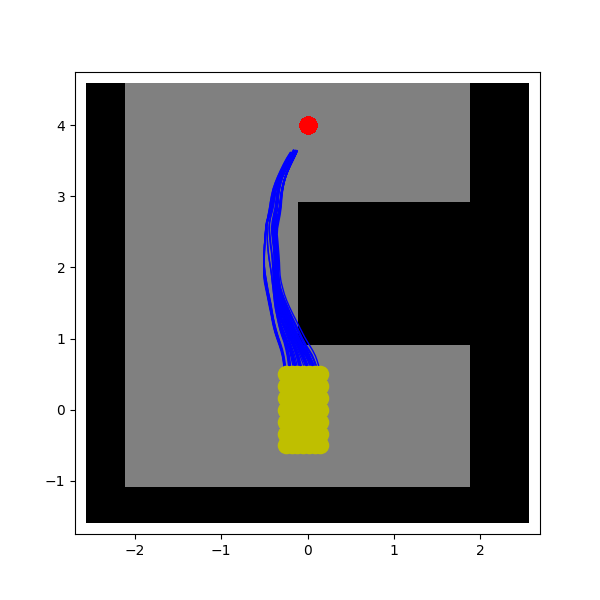
\includegraphics[width=\textwidth, height=3.5cm, trim={0cm 1cm 0cm 1cm},clip]{Figures/Chapter_CPSB/hole_LEAS-P2.png}
        \caption{LEAS-P2}
    \end{subfigure}
    \caption{Scenario B1 (hole): initial configurations succeeding (yellow dot) and failing (magenta dot) with SBCP.}
    \label{fig:cp-sb:trajectories_hole}
\end{figure}


\begin{figure}[h!]
    \captionsetup[subfigure]{justification=centering}
    \centering
    \begin{subfigure}[t]{0.32\linewidth}
        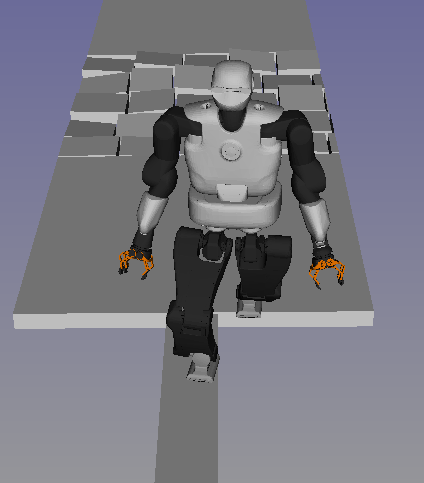
\includegraphics[width=\textwidth, height=5cm]{Figures/Chapter_CPSB/talos_bridge_kino.png}
        \caption{}
        \label{fig:cp-sb:talos_configurations_hole_bridge_block0}
    \end{subfigure}
    \begin{subfigure}[t]{0.32\linewidth}
        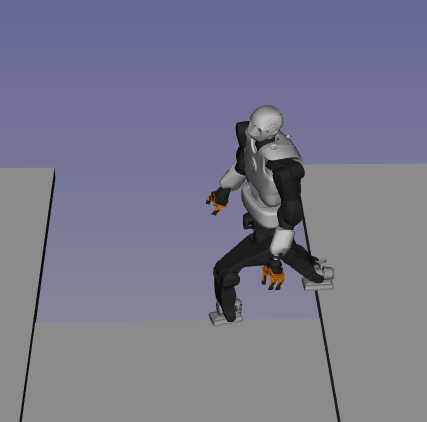
\includegraphics[width=\textwidth, height=5cm]{Figures/Chapter_CPSB/talos_hole_kino.png}
        \caption{}
        \label{fig:cp-sb:talos_configurations_hole_bridge_block1}
    \end{subfigure}
    \begin{subfigure}[t]{0.32\linewidth}
        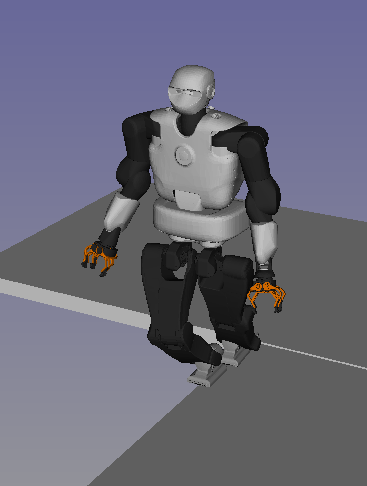
\includegraphics[width=\textwidth, height=5cm]{Figures/Chapter_CPSB/talos_hole_not_good.png}
        \caption{}
        \label{fig:cp-sb:talos_configurations_hole_bridge_unfeasible}
    \end{subfigure}
    \caption{Scenario B1: (a)(b) blocking Talos configurations above the void  and (c) configuration valid but unfeasible on the real robot.}
    \label{fig:cp-sb:talos_configurations_hole_bridge}
\end{figure}


% What is tested
\paragraph{Scenario B1 - Hole and Bridge.} 
We compute contact sequences on guide paths generated by our steering methods on the hole and bridge scenarios (Figure \ref{fig:cp-sb:scenarios_hole_bridge}). 
These two scenarios are similar as they can both lead to weak contact configurations located very close to the edge of the obstacles that are unfeasible by the robot in reality (Figure \ref{fig:cp-sb:talos_configurations_hole_bridge}).
We evaluate for both terrains the success rate with the contact planner and measure the average $robustness$ of the configurations in contact when passing near the obstacle.
% What is the robustness used for
The robustness quantifies how far the center of mass of the robot is from the boundaries of the friction cones of the contact forces, giving us a measure of the static equilibrium of one robot configuration (we refer the reader to \cite{AcyclicCP} for further details).
% We first give a linear program (LP) that verifies whether a contact configuration allows for static equilibrium. This LP is the same that was proposed in [32]. 
% From this formulation we derive a new LP that quantifies the robustness of the equilibrium to uncertainties in the contact forces. In turn, from this value we can either choose the most robust candidate, or set a threshold on the required robustness.
In this work, we use the measure of the robustness to give us an overall estimation of the stability of the contact plan generated, where a lower value means a more difficult guide path in the input of the contact planner (i.e. too close to the obstacles, too high or low...) leading to unstable configurations in contact.
Conversely, a high robustness value should be the result of a \qq{good} feasible guide path.
%\textcolor{blue}{STEVE: est-ce que c'est bon comme explication ou j'ai tout faux / faut ajouter plus.}

 


% Initialization
We uniformly sample some initial configurations on a small area from where all our steering methods can generate valid guide paths ($\tilde{\mathcal{R}^*}$ and $\tilde{\mathcal{C}}$) up to the target.
We set each initial robot configuration oriented toward the target, located on the other side of the obstacle, with an initial velocity $||v||=0.04$ m/s.
% Where are the results
Results are shown in Table \ref{tab:cp-sb:hole_bridge} with SBCP success rate for both bridge and hole scenarios. Figure \ref{fig:cp-sb:trajectories_hole} shows generated trajectories on the hole scenario.


% RB-Kino and RB-Lin
Results show that RB-Lin and RB-Kino generate valid guide paths up to the goal, but do not consider the terrain, resulting in configurations passing close to the void. As a consequence, these guide paths lead to a low success rate and some weakly robust contact plans on both terrains.

% LEAS-P1 and LEAS-P2
In comparison, LEAS-P1 and LEAS-P2 generate guide paths with a strong hole avoidance behavior leading to a higher success rate and more robust configurations in both scenarios.
LEAS-P1, trained without contact planner feedback, performs well in these scenarios where the stricter reachability constraint $\tilde{\mathcal{R}^*}$ encourages to keep the robot root above the ground while keeping a safe margin of error. 
As a result, trajectories of LEAS-P1 tend to be further from the hole than RB-Kino and RB-Lin (Figure \ref{fig:cp-sb:trajectories_hole}). 
However, we can still notice some successful guide paths with weakly robust configurations that are unfeasible on the real robot (Figure \ref{fig:cp-sb:talos_configurations_hole_bridge_unfeasible}).
In contrast, the results of LEAS-P2 demonstrate how it can produce guide paths staying even further from the hole, thus generating more robust configurations and increasing the contact planning success rate.

% About the robustness
Results in Table \ref{tab:cp-sb:hole_bridge} show that there is a correlation between the contact planning success and the robustness measured. This is expected as SBCP from an unstable configuration often fails to generate a new contact to reach the next root position on the guide.
%\stn{ca sort d ou ces termes ?} \textcolor{blue}{En effet j'ai oublié de les enlever.}
%\textcolor{red}{La robustness permet d'avoir une idée de la pertinence des configs, mais pas tellement non plus. Il faudrait une meilleure mesure.}
However, we also notice that this correlation is not pertinent for all scenarios, like the bridge where RB-Kino presents a high robustness score close to LEAS-P2 but the worst success rate among our steering methods. 
Indeed some configurations can be selected as the most robust but they may not permit the generation of a new contact (Figure \ref{fig:cp-sb:talos_configurations_hole_bridge_block0} and \ref{fig:cp-sb:talos_configurations_hole_bridge_block1}).

We have shown in the hole and bridge scenarios how LEAS-P2 learns to increase the success rate of the contact planner and indirectly improve the robustness of the contact plan through its validation during the training.
%It thus learns what makes a feasible guide path for it.
% with an emphasis on the reachability condition $\tilde{\mathcal{R}^*}$,

%This highlights the limitations of our previous steering that do not consider approximate well the capabilities of the robot on the contact planner, 
%but also the efficacy of using heuristics based on the robustness measure for the sample selection during the contact generation. 
%\textcolor{red}{Not really true, so I may remove it. Steve if you can give an input on that. On how to formulate all that.} \stn{je m emmerderais pas trop avec le robustness la, tu l as meme pas mise dans ton cout. je dirais juste en side effect que t as tendance a generer des configs plus robuste si c est le cas mais la tu dis rien de ocmment tu recuperes cette valeur et ce qu elle representent}

\paragraph{Scenario B2 - Wall.}
% It learns the constraint hand-wall.

% What did we do to evaluate that
We now evaluate on the wall scenario what kind of additional constraints LEAS can learn from the contact planner. In the wall scenario, LEAS must focus on generating a collision-free guide path ($\tilde{\mathcal{C}}$).
%and compute the contact sequence along it with SBCP.
Results are shown in Figure \ref{fig:cp-sb:talos_wall}.
% Results
As the original collision volume (i.e. the trunk) does not include the hands of the robot, guide paths generated by LEAS-P1 (a) pass very close to the wall and fail with SBCP as for the given root position and orientation, a collision occurs between the hand of Talos and the wall (Figure \ref{fig:cp-sb:talos_wall:p1}).
In contrast, LEAS-P2 (b) learned during the training how to avoid such collision with the hand by rotating the robot (Figure \ref{fig:cp-sb:talos_wall:p2}).
We note an interesting behavior where LEAS balances the rewards $R_{ori}$ and $R_{dir}$, to keep its orientation and to move toward the target respectively, with the contact planning constraints, hence making the robot sidewalk along the wall while keeping it in its visual field.

% Previous paper LEAS-P1/LEAS-P2 => No stricter constraint on validation.
We reproduced a similar experiment in our original work \cite{LEAS}, learning LEAS with $\tilde{\mathcal{R}}$ (i.e. without the stricter constraint to lie above the ground, cf. previous chapter), thus leading LEAS-P1 to have the same success rate than RB-Lin and RB-Kino on the hole and bridge scenarios (Table \ref{tab:cp-sb:hole_bridge}).
% So we trained with P2
Then we trained LEAS-P2 with this same reachability condition $\tilde{\mathcal{R}}$, plus feedback from the contact planner.
As expected, the policy learned to move the robot while keeping a safe distance from the void and reached the same success rate as our actual version of LEAS-P1 and LEAS-P2 trained with the stricter reachability condition $\tilde{\mathcal{R}^*}$.

% What was the pbm and why not keep that
These experiments demonstrate what kind of behaviors LEAS can learn to generate feasible guide path by our contact planner. 
From these results, we decided to implement these constraints directly inside the validation function: first, the stricter constraint to force the robot to lie above the ground $\tilde{\mathcal{R}^*}$ (already implemented in the results), then extending the collision volume of the robot to include its hand positions when its arms are attached.
%and depending on its fixed default hand configurations $[L^{hand\_left},L^{hand\_right}]$.
% Also done in hpp-rbprm: larger rom for collision or the "s" parameter
%Such constraint was already introduced in \cite{AcyclicCP} where they tune a scaling parameter $s$ to widen the volume of the robot trunk or manually design the collision volume to include the robot hands.
% Consequence
While reducing the feasibility space of the generated guide paths, these approximations greatly accelerate the training ($\approx 20-30$\%) as the guide paths generated are subject to tighter validity constraints (i.e. root above the ground and with less probability of collisions), thus resulting in a faster contact generation.


\begin{figure}[h]
    \captionsetup[subfigure]{justification=centering}
    \centering
    \begin{subfigure}[t]{0.48\linewidth}
        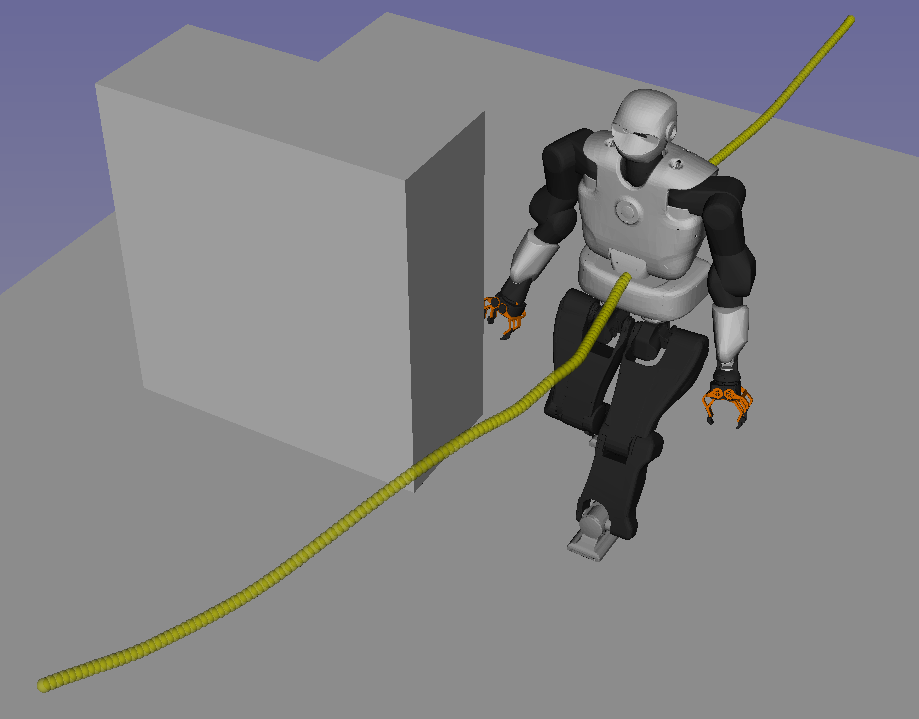
\includegraphics[width=\textwidth, height=5cm]{Figures/Chapter_CPSB/avoid_wall_fail.png}
        \caption{LEAS-P1: Collision\label{fig:cp-sb:talos_wall_collision}}
        \label{fig:cp-sb:talos_wall:p1}
    \end{subfigure}
    \begin{subfigure}[t]{0.48\linewidth}
        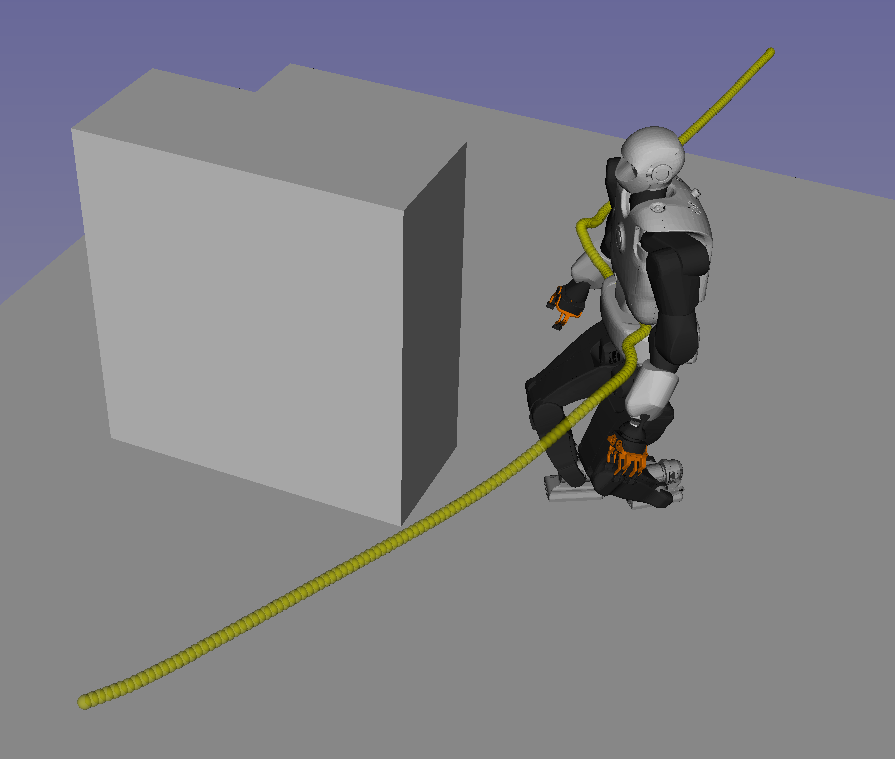
\includegraphics[width=\textwidth, height=5cm]{Figures/Chapter_CPSB/avoid_wall.png}
        \caption{LEAS-P2: Avoid the contact\label{fig:cp-sb:talos_wall_ok}}
        \label{fig:cp-sb:talos_wall:p2}
    \end{subfigure}
    \caption{Scenario B2: (a) LEAS-P1 collision of the robot hand with the wall, (b) LEAS-P2 rotates the robot to avoid a such collision.}
    \label{fig:cp-sb:talos_wall}
\end{figure}


\subsection{Scenario C: Uneven Terrains}
% Rubbles
\begin{figure}[H]
    \captionsetup[subfigure]{justification=centering}
    \centering
    \begin{subfigure}[t]{0.4\linewidth}
        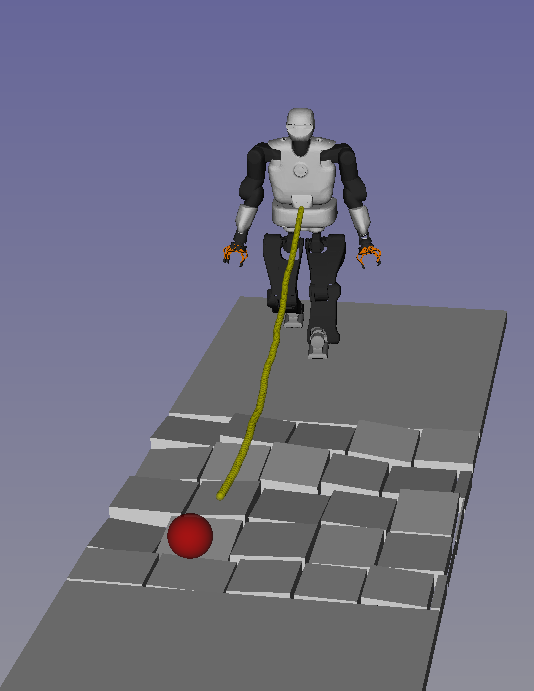
\includegraphics[width=\textwidth, height=6cm]{Figures/Chapter_CPSB/rubbles_0.png}
    \end{subfigure}
    \begin{subfigure}[t]{0.4\linewidth}
        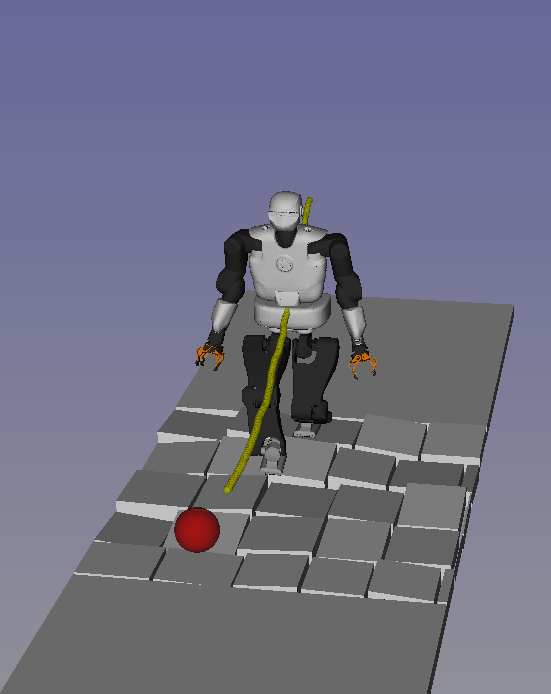
\includegraphics[width=\textwidth, height=6cm]{Figures/Chapter_CPSB/rubbles_1.png}
    \end{subfigure}
    \begin{subfigure}[t]{0.4\linewidth}
        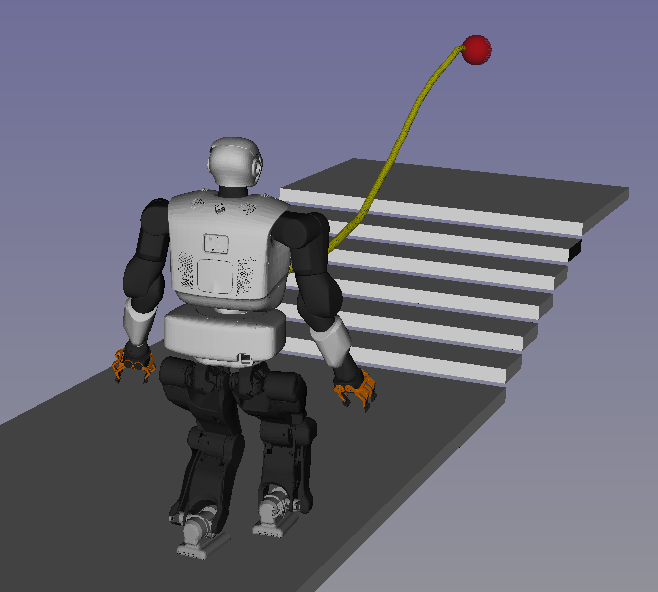
\includegraphics[width=\textwidth, height=5cm]{Figures/Chapter_CPSB/stairs_diago.png}
    \end{subfigure}
    \begin{subfigure}[t]{0.4\linewidth}
        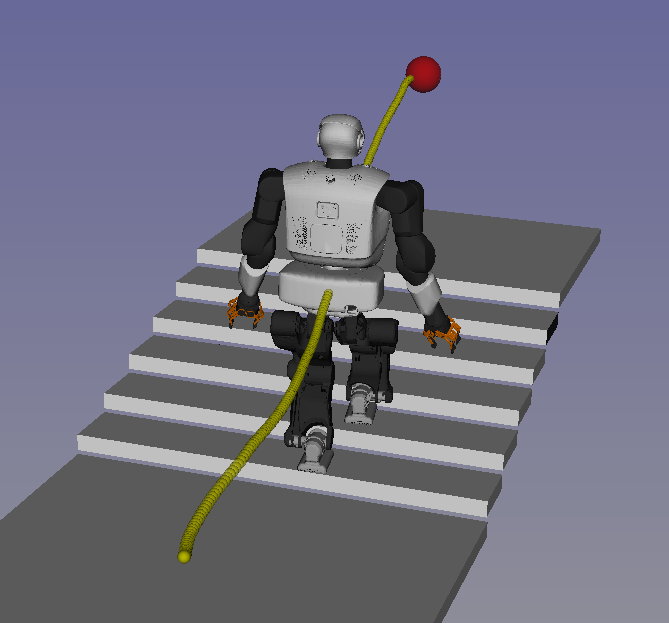
\includegraphics[width=\textwidth, height=5cm]{Figures/Chapter_CPSB/stairs_diago1.png}
    \end{subfigure}
    \caption{Scenario C: Contact planning on rubbles and stairs scenarios, with (yellow) the guide path generated by LEAS-P2 and (red) the goal.}
    \label{fig:cp-sb:talos_stairs_rubbles_example}
\end{figure}
% What scenarios are tested here
We now present a comparison on two complex terrains: the stairs and the rubbles.
% What were the results on the previous paper for these scenarios
In \cite{AcyclicCP}, these scenarios were easily solved using the steering methods RB-Lin and RB-Kino with a near $100$ \% success rate. 
However, these tests were performed for a reduced set of initial configurations starting directly in front of the obstacle and oriented toward it. 
%\textcolor{blue}{Nicolas: We later observed that the same planners only lead to limited results when the initial conditions vary (e.g. when the robot initial orientation is less favorable). Answer: Je trouve que la phrase n'apporte pas grand chose et on ne parle pas d'orientation dans ce scenario.}
% Why do we redo it here
In this work, we extend these tests on a wider range of initial configurations with RB-Kino (with RRT path planning if required), LEAS-P1 and LEAS-P2. Then we measure their success rate and the robustness of the contact plans generated when crossing the terrain.
For all our tests, we orient the robot directly toward the target with an initial velocity of $v=0.04$ m/s. \hfill \break

\begin{table}[h]
\centering
\caption{Scenario C: Comparison on the success rate and robustness. \label{tab:SBCP:rubbles_robustness}}
\begin{tabular}{ |c|c|c|c|c| }
    \hline
    Parameters & Terrains & RB-Kino+RRT & LEAS-P1 & LEAS-P2\\
    \hline \hline
    \multirow{3}{*}{SR} & Rubbles & 100\% & 100\% & 100\% \\
    \cline{2-5}
                        & Stairs & 74\% & 100\% & 100\% \\
    \hline \hline
    \multirow{3}{*}{Robustness} & Rubbles & 30.4 & 24.9 & 26.45 \\
    \cline{2-5}
                                & Stairs  & 24.3 & 28 & 33.2 \\
    \hline
\end{tabular}
\label{tab:cp-sb:rubbles_stairs}
\end{table}

\paragraph{Scenario C1 - Rubbles.}
% Do it on rubbles of 1x11 => This was not a problem in the acyclic paper. 
% We expected a lot of repositioning but no: the samples + the heuristics chosen are very good.
% No real difference between all SM, the robustness is smaller on LEAS compared to lin and kino ? Why ?
% But it does not change anything on the success.
% But LEAS is a bit lower on z than the other SM => Is that why ?
%\textcolor{red}{This test is very small, we do not see much here. It always work with SBCP and the robustness does not mean much. The only thing I could talk about is the contact plan quality that is not good at all visually, but it's not really my topics.}
Starting from a flat ground area and oriented toward the obstacle, the robot has to cross some small uneven surfaces with different heights and orientations and reach a fixed target on the other side (Figure \ref{fig:cp-sb:talos_stairs_rubbles_example}).
% Results
Results in Table \ref{tab:cp-sb:rubbles_stairs} show no difference between RB-Kino which does not require path planning to succeed in this scenario, LEAS-P1, and LEAS-P2. All three steering methods present a success rate of $100$\% with SBCP, thus matching the results presented in \cite{AcyclicCP}.
% Why these results on robustness
However, we can note a lower robustness score for LEAS-P1 and LEAS-P2, which we explain by the difference in height of the root configurations along the guide path that tends to be lower on LEAS with an average root height of $z=0.86$ meters from the ground compared to RB-Kino that keeps a constant height $z=0.95$ all along the trajectory.
On the rubble scenario, lower configurations present a lesser robustness score but do not impact the success rate.

% What can we conclude
We can conclude that the rubble scenario is easily solved by the contact planner for any guide path generated by our steering methods. 
In the future, it could be interesting to focus more on the guide discretization step that is on average equal to $\Delta D \approx10$ cm here. In this scenario, learning with LEAS how to generate guide paths with a higher $\Delta D$ and successful with SBCP, could improve the computation time as well as the quality of the contact plans. %\hfill \break

%\textcolor{red}{Put a picture to show the trajectories of RB-Kino vs LEAS-P1 vs LEAS-P2, to show the difference. They all work, 100\% success rate.}

% What can I conclude about SBCP on rubbles
%\textcolor{red}{I do not know if LEAS learned something here. It learned to stay lower to have a bigger margin on collision / reachability but that's all probably ? SBCP always work here anyway for these samples and heuristics.}

\paragraph{Scenario C2 - Stairs.\label{sec:cp-sb:par:stairs}}

We present a comparison of RB-Kino, RB-Kino(+RRT), LEAS-P1, and LEAS-P2 on a wide range of initial configurations for the stairs scenario (Figure \ref{fig:cp-sb:talos_stairs_rubbles_example}).
We evaluate our steering methods with SBCP on the stairs for the climbing up task only, as in our experiments the climbing down task was presenting similar results and limitations.

% RB-Kino and why RRT
As presented in Figure \ref{fig:cp-sb:stairs_sm_kino}, RB-Kino succeeds to generate valid guide paths only when placed directly in front of the stairs and where further initial configurations lead to configurations unable to reach the ground (invalid with $\mathcal{R}$). 
For a broader comparison, we plug RB-Kino into a path planning algorithm (RRT) to compute valid guide paths from all previously failed configurations by RB-Kino.
We can note in Figure \ref{fig:cp-sb:stairs_sm_kino_rrt} that the intermediate waypoints found to solve this simple scenario are far from efficient.

% Success rate
Results in Table \ref{tab:cp-sb:rubbles_stairs} show that the success of RB-Kino+RRT suffers from a limitation, also hinted by with RB-Kino without RRT, where guide paths with configurations at the limit of the reachability condition $\mathcal{R}$ can lead to failed contact plans with SBCP (magenta dots in Figure \ref{fig:cp-sb:stairs_sm}).
Some contact configurations resulting from a too high and too low guide path are shown in Figure \ref{fig:cp-sb:stairs_difficult}, where no transition is feasible from the actual root position to the next.
In order to avoid guide paths at the limit of the reachability condition, RB-Kino requires a manual selection of the initial configuration or manually added waypoints at the bottom of the stairs to succeed with SBCP.

\begin{figure}[ht]
    \captionsetup[subfigure]{justification=centering}
    \centering
    \begin{subfigure}[t]{0.48\linewidth}
        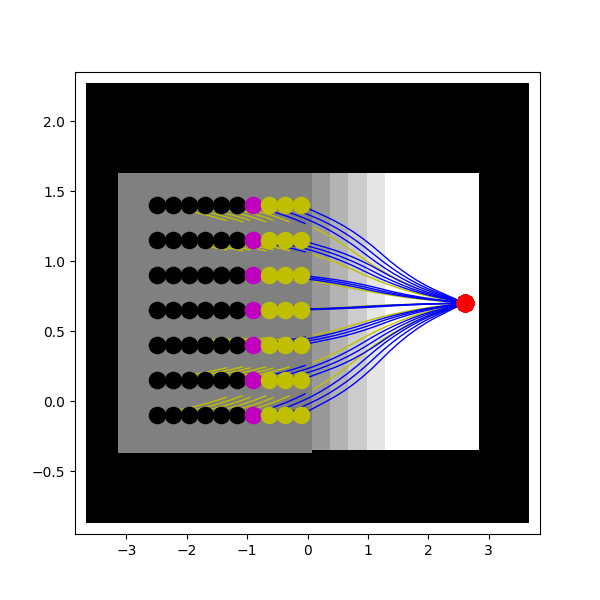
\includegraphics[width=\textwidth, height=5cm]{Figures/Chapter_CPSB/stairs_kino.png}
        \caption{RB-Kino\label{fig:cp-sb:stairs_sm_kino}}
    \end{subfigure}
    \begin{subfigure}[t]{0.48\linewidth}
        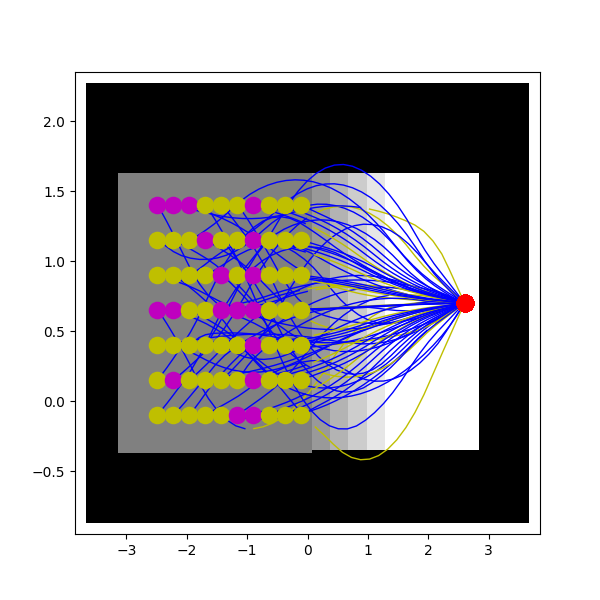
\includegraphics[width=\textwidth, height=5cm]{Figures/Chapter_CPSB/stairs_kino_rrt.png}
        \caption{RB-Kino + RRT\label{fig:cp-sb:stairs_sm_kino_rrt}}
    \end{subfigure}
    \begin{subfigure}[t]{0.48\linewidth}
        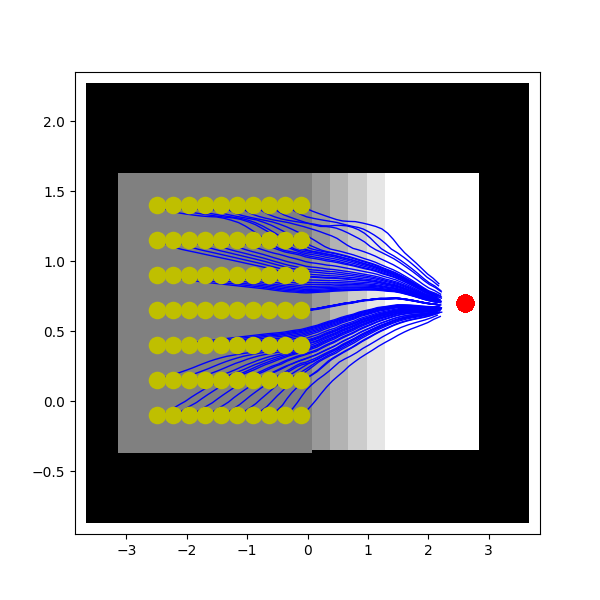
\includegraphics[width=\textwidth, height=5cm]{Figures/Chapter_CPSB/stairs_leas_p1.png}
        \caption{LEAS-P1}
    \end{subfigure}
    \begin{subfigure}[t]{0.48\linewidth}
        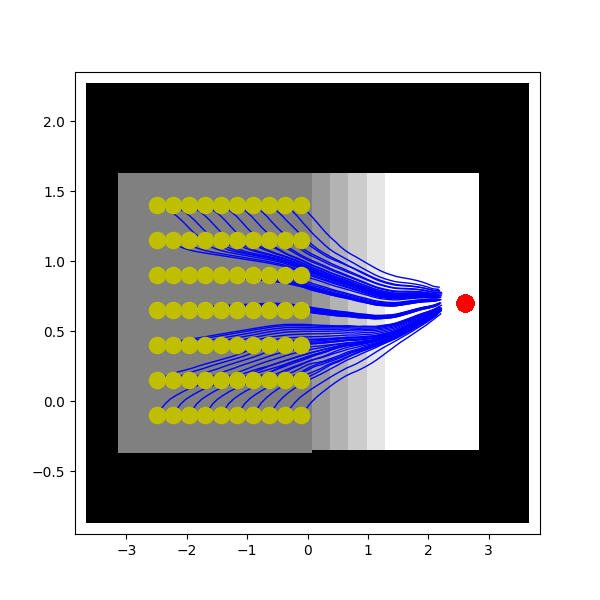
\includegraphics[width=\textwidth, height=5cm]{Figures/Chapter_CPSB/stairs_leas_p2.png}
        \caption{LEAS-P2}
    \end{subfigure}
    \caption{Scenario C2: initial configuration with guide path (yellow dot) valid and successful with SBCP, (magenta dot) valid but failing with SBCP, (black dot) invalid and (red dot) the target.}
    \label{fig:cp-sb:stairs_sm}
\end{figure}

In comparison, the steering methods LEAS-P1 and LEAS-P2 succeed without path planning to reach the target and to compute a contact sequence with SBCP from all initial configurations.
% Why ?
An advantage of using deep RL to learn such a steering method is that the policy is encouraged to stay far from the critical states (near the reachability condition limits) and thus avoids implicitly difficult and blocking configurations with our contact planner.
% Relation robustness / success
We denote the same correlation between the robustness score and the success rate (Table \ref{tab:cp-sb:rubbles_stairs}) as our previous test scenarios, and how LEAS-P2 learns to generate guide paths fitting SBCP, leading to more robust contact plans than LEAS-P1 and RB-Kino.

% Analysis
To better evaluate what makes a good guide path for this contact planner on the stairs scenario, we average all the guide paths generated on stairs and render the averaged trajectory on the vertical plane (Figure \ref{fig:cp-sb:stairs_xz}).
% Kino+RRT
As previously hinted, results show that RB-Kino+RRT tends to engage the stairs with a higher root height and to climb with a lower root position compared to LEAS-P1 and LEAS-P2, thus leading to difficult contact configurations (Figure \ref{fig:cp-sb:stairs_difficult}).
% LEAS-P1 and LEAS-P2
On the other hand, LEAS-P1 and LEAS-P2 tend to keep the root of the robot at a constant distance from the ground and produce some more robust contact plans.
% Difference between both LEAS-P1 and LEAS-P2
A comparison of the robustness score between LEAS-P1 and LEAS-P2 is complex as the difference between their trajectories is subtle. 
However, we can notice that LEAS-P1 and LEAS-P2 tend to keep a constant distance from the ground, on average $90$ cm and $94$ cm respectively (maximum distance root-ground with Talos is $105$ cm), which explains the difference in robustness.

\begin{figure}[h]
    \centering
    \begin{subfigure}[t]{0.42\linewidth}
        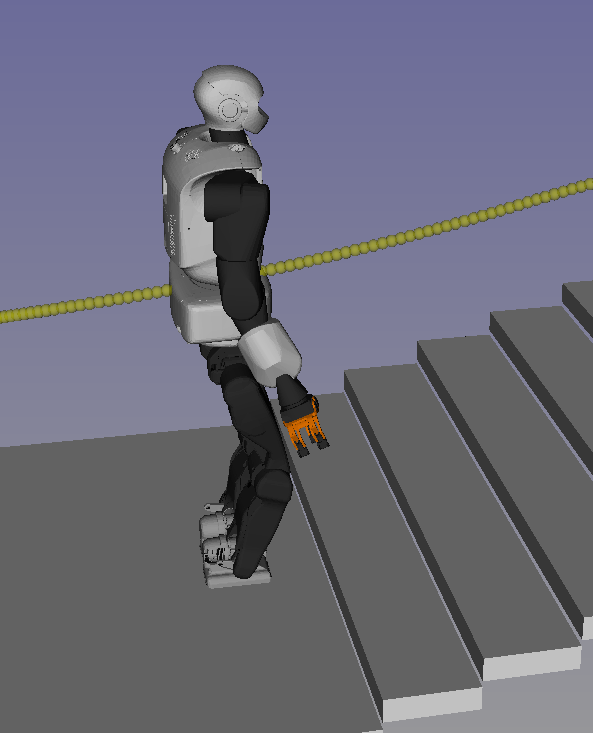
\includegraphics[width=\textwidth, height=6cm]{Figures/Chapter_CPSB/stairs_too_high_2.png}
        \caption{\label{fig:cp-sb:stairs_difficutl_high}}
    \end{subfigure}
    \begin{subfigure}[t]{0.42\linewidth}
        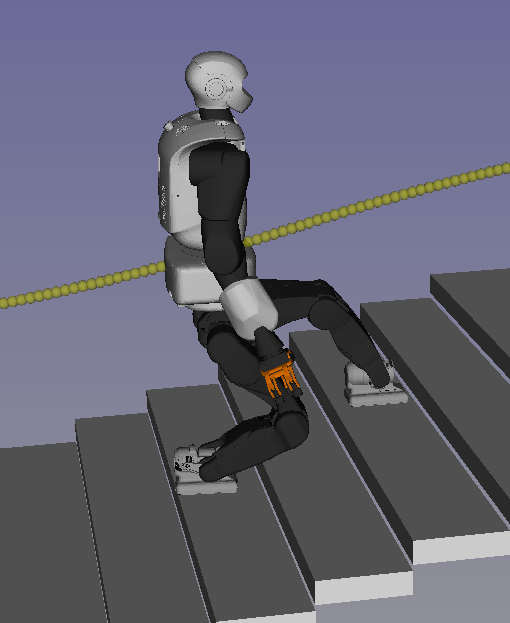
\includegraphics[width=\textwidth, height=6cm]{Figures/Chapter_CPSB/stairs_too_low.png}
        \caption{\label{fig:cp-sb:stairs_difficutl_low}}
    \end{subfigure}
    \caption{Scenario C2: Difficult root configuration on the guide for SBCP: (a) too high where the robot has its legs in extension and can not reach the next root position, (b) too low where the robot climbs the stairs crouched.}
    \label{fig:cp-sb:stairs_difficult}
\end{figure}
\begin{figure}[h]
    \centering
    \begin{tikzpicture}
        \node at (1,1) {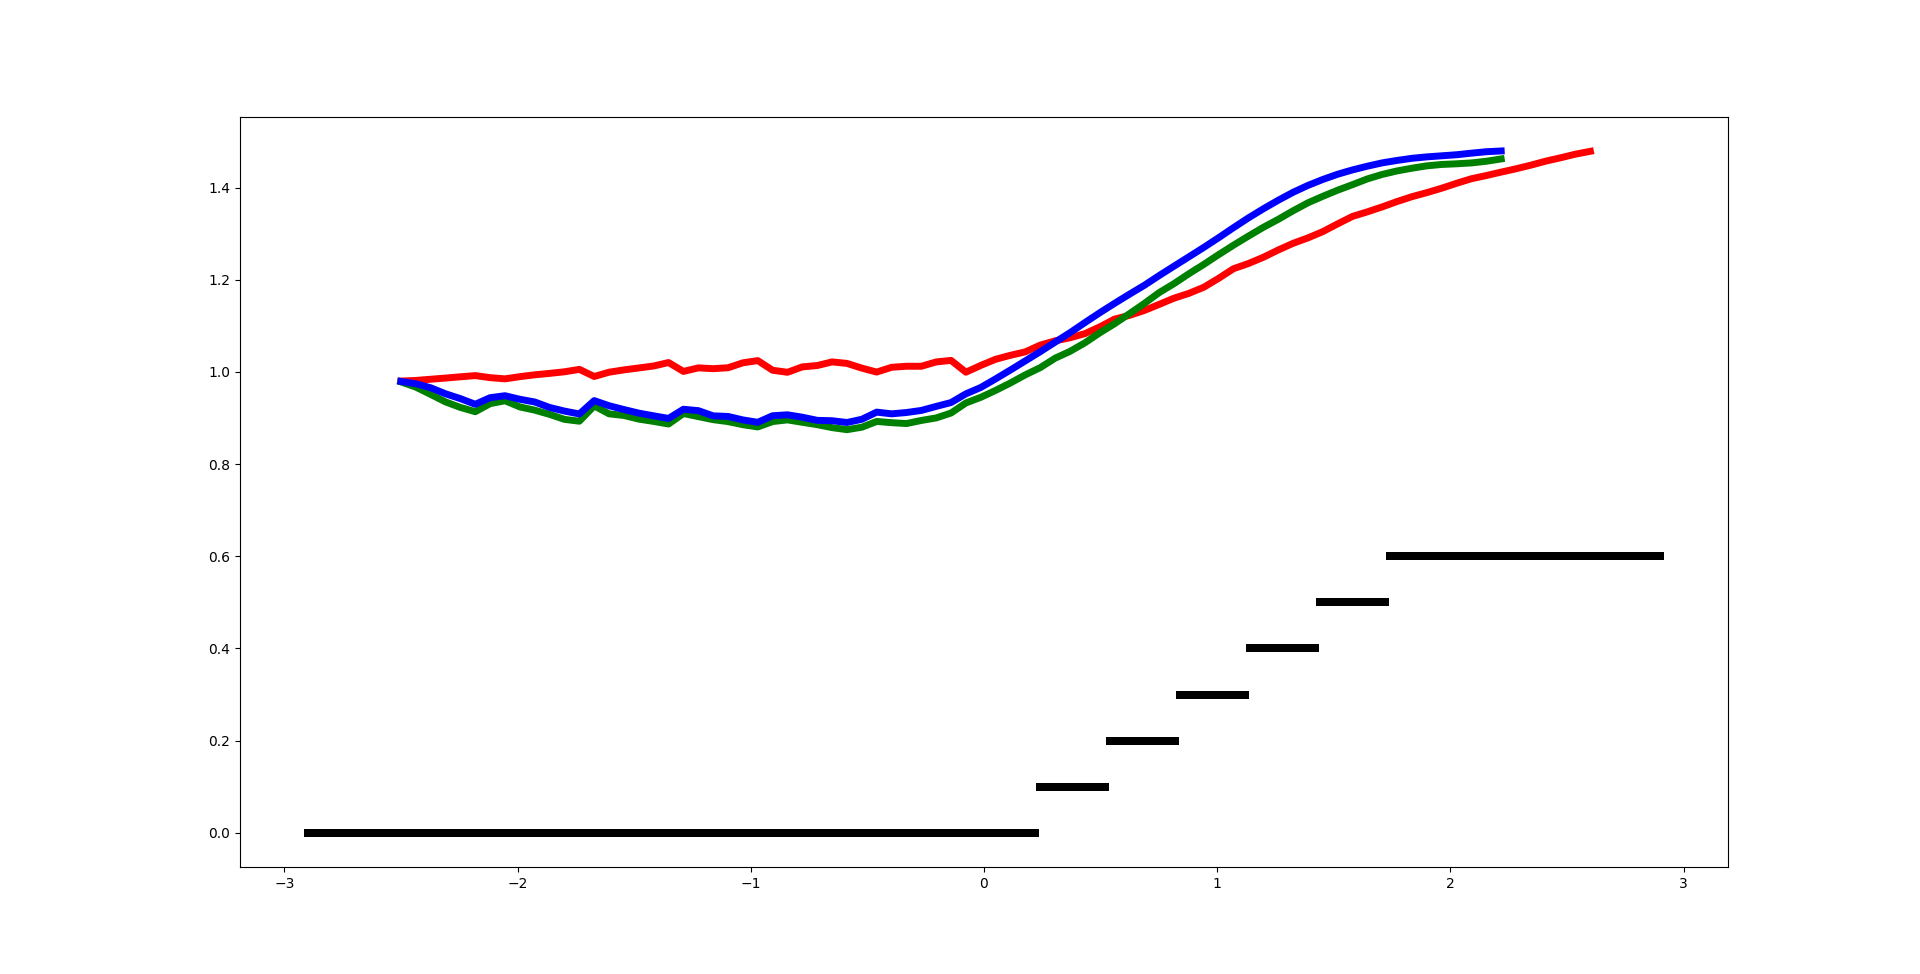
\includegraphics[trim={2cm 2cm 2cm 2cm}, clip,width=\textwidth, height=6cm]{Figures/Chapter_CPSB/stairs_z.png}};
        \node at (5.5,-1) {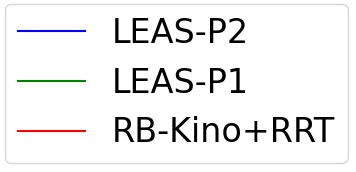
\includegraphics[width=0.18\textwidth]
        {Figures/Chapter_CPSB/legend_height_chap_p2.png}};
    \end{tikzpicture}
    \caption{Stairs scenario: guide path comparison on z-axis generated by LEAS-P1, LEAS-P2 and RB-Kino+RRT.}
    \label{fig:cp-sb:stairs_xz}
\end{figure}


\section{Discussion\label{sub:cp-sb:discussion}}

\subsection{Implementation Choices}
% === Behaviour and experiments
\begin{figure}[h]
    \centering
    \begin{subfigure}[t]{0.19\linewidth}
        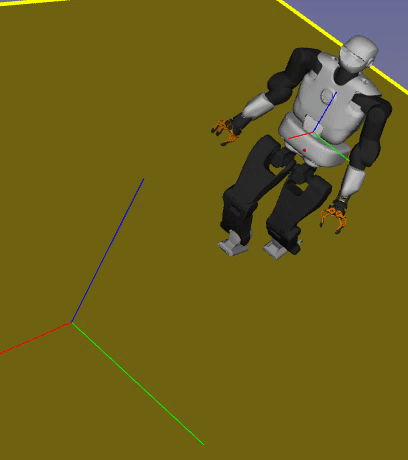
\includegraphics[width=\textwidth,trim={3cm 3cm 0 0}, clip] {Figures/Chapter_CPSB/sidewalk_seq/frame_0.png}
    \end{subfigure}
    \begin{subfigure}[t]{0.19\linewidth}
        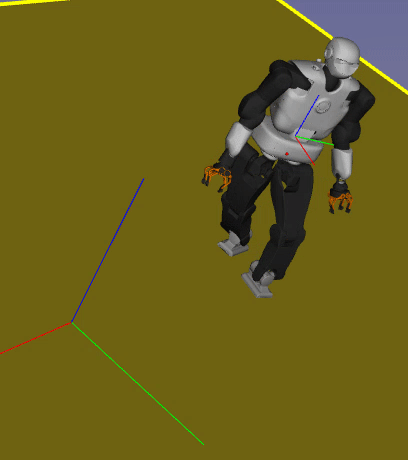
\includegraphics[width=\textwidth,trim={3cm 3cm 0 0}, clip] {Figures/Chapter_CPSB/sidewalk_seq/frame_1.png}
    \end{subfigure}
    \begin{subfigure}[t]{0.19\linewidth}
        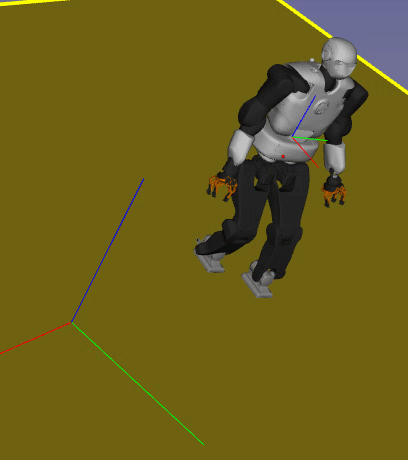
\includegraphics[width=\textwidth,trim={3cm 3cm 0 0}, clip] {Figures/Chapter_CPSB/sidewalk_seq/frame_2.png}
    \end{subfigure}
    \begin{subfigure}[t]{0.19\linewidth}
        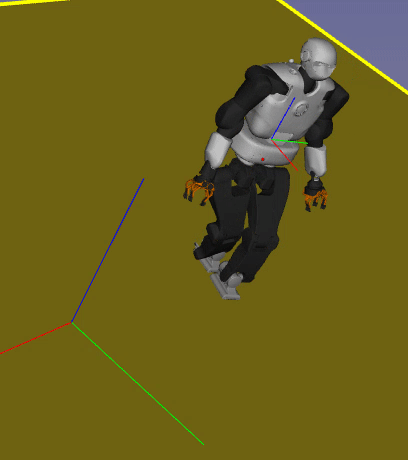
\includegraphics[width=\textwidth,trim={3cm 3cm 0 0}, clip] {Figures/Chapter_CPSB/sidewalk_seq/frame_3.png}
    \end{subfigure}
    \begin{subfigure}[t]{0.19\linewidth}
        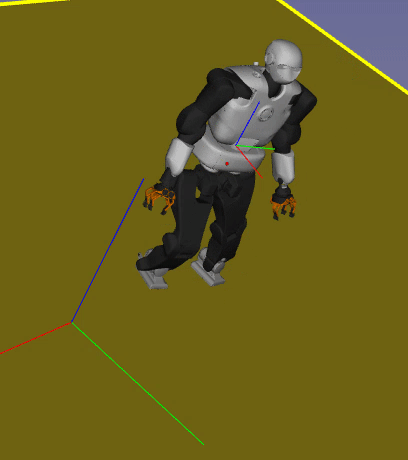
\includegraphics[width=\textwidth,trim={3cm 3cm 0 0}, clip] {Figures/Chapter_CPSB/sidewalk_seq/frame_5.png}
    \end{subfigure}
    \caption{Without reward on the orientation, LEAS-P2 learns that the sidewalking strategy is the most robust and successful with SBCP.}
    \label{fig:cp-sb:sidewalk_seq}
\end{figure}

%In this work, we made several implementation choices impacting the contact planning.

% - SIDEWALKING -
\paragraph{Constraint on the orientation.}
In LEAS design, the reward $R_{ori}$ penalizes the agent for not orienting the robot toward the goal. 
As discussed previously, this design choice can be limiting in cluttered environments where sidewalking is required, but we decided it was necessary.

In our first design, we initially trained LEAS-P2 without this reward on the orientation, expecting it to learn that a straight walk is the best strategy (i.e. moving while being oriented toward the goal). 
However, the result was as shown in Figure \ref{fig:cp-sb:sidewalk_seq}, where LEAS discovered that the most successful approach to plan contacts was by sidewalking.
Experiments on our other terrains led to the same result. 
From a higher level perspective, this strategy makes sense as humans do it too, to walk on complex terrains where they require more stability (e.g. crossing a narrow bridge or climbing down stiff stairs).

However, sidewalking is not the behavior we desire for our biped robot locomotion task and as a consequence, we decided to penalize it on LEAS with $R_{ori}$. We tuned the associated weight $w_{ori}$ to balance this penalty and the behavior learned to succeed in the contact planning, as previously shown on the wall scenario B2 (\ref{fig:cp-sb:talos_wall_ok}) where the robot sidewalks to avoid the collision and walk straight on the rest of path. However, this reward design may not be suitable for other scenarios and has to be explored in more detail.

\paragraph{Guide discretization for LEAS.\label{par:cpsb:discussion_guide_discretization}}
With the desired velocity $v_{desired}$ and the timestep $T$ set in LEAS, we obtain an average discretization step (i.e. distance between each root configuration) on the guide of $\Delta D=2$cm. 
As shown in section \ref{subsub:cp-sb:tradeoff}, such a low value presents the best success rate with our contact planner at the cost of a high number of steps in the contact plan, and so a high computation time. We aim for a value $\Delta D=10$cm for the guide paths in the input of SBCP, that offers a suitable trade-off.
Such value is easily reached in RB-Kino and RB-Lin, which generate guide paths as a function of the time $G=f(t)$, by increasing the timestep $T$.
LEAS could also directly achieve such a discretization step with the same strategy.
However, a higher timestep leads to actions with a bigger impact on the system, more probability to meet a critical state and so, a less stable learning overall.
Another point to consider is the impact of such change on the reward, and so the navigation results presented in the previous chapter and the need to retrain a new policy for this new timestep value.

That is why we opted for a less intrusive method by further discretizing the guide generated by LEAS, keeping 1 out of 5 five root configurations on it, resulting in $\Delta D=2 \times 5=10$cm.
This enabled us to use the same policy LEAS-P1 for our comparisons, trained in the previous chapter, and to retrain a new policy from scratch, LEAS-P2, on the same reward basis but adding the contact planning validation (P2).

%\textcolor{blue}{CHECK WHAT I WROTE HERE AND CORRECT}
A question one could ask is if a fixed discretization step $\Delta D$ along the guide is desirable. 
Indeed, we saw that the tuning of this value presents a trade-off on our contact planner where it can be pertinent to set a small $\Delta D$ for complex sections of the guide path to increase its success (e.g. egress scenario where going out of the car required a value $\Delta D=3$ cm in \cite{AcyclicCP}), or adjust it to a higher value on easier sections where the contact planner is almost sure to succeed (e.g. walking on flat ground with $\Delta D=15$ cm).
% Expe
%We trained such policies by increasing the discretization step to $\Delta D = 20$ cm, by keeping 1 out of 10 configurations along the guide.
%LEAS had to navigate the terrain at the desired velocity, while succeeding in the contact planning. As such a value would not be achievable on complex terrains, LEAS had to lower its velocity to succeed.
%However, this strategy was intractable in practice due to the high contact planning time required on guide paths with $\Delta D > 15$cm.
%Indeed, reaching a far root configuration often requires a stabler initial contact configuration, where repositioning can help at the cost of a higher computation time (higher number of footsteps).
%Such computation time was not clearly apparent in our previous analysis on the discretization on stairs (Section \ref{subsub:cp-sb:tradeoff}). Indeed, further experiments on stairs have shown that when failing a contact generation, further repositioning of limbs in contact did not help and directly led to a failure, thus stopping the computation.
%In comparison, it was not the case on other terrains, especially in the hole scenario where such repositioning was intensively used on configurations near the surface edges leading to an exponential computation time.
% Our choice
On this contact planner, we made the choice to aim for a fixed discretization step $\Delta D=10$ cm to balance computation time and success rate.
However, having a variable discretization depending on the terrain is the most pertinent extension of this work in terms of computation and quality of contact plan with SBCP.
This problem will be further investigated in Chapter \ref{sec:CP-SL1M} on a different contact planner.

%\paragraph{Heuristics and Robustness}
%As we have seen in the results, the choice of the heuristics defined in the contact planner is another critical parameter.
%However in this work we used SBCP as a black-box, and we did not further investigate the impact of other heuristics at our disposal on our results.
%Another parameter we could have investigated is the robustness treshold

% === Learning
% D - Other learning strategies ? Now it's pruning the failing traj. 
% We can add a reward function of the robustness, it's close to the traversability kinda saying that a guide/path is difficult or not. And it would require more reward engineering.
% We can use a sparse reward just to learn how to cross a link, far less general and would require other methods as HER etc.
% E - Pretraining for demonstration with trajectories of LEAS-P1. Catastrophic forgetting with PPO => Imitation learning, Continual learning, learning from demonstration etc...
\subsection{Learning Strategy}
% Is pruning the failing trajectory really the best choice for learning.
To learn how to generate guide paths fitting the contact planner, one could ask if the strategy of pruning the failing part of the trajectory is the best and if some alternatives exist.
We thought of several reward designs to learn from the feedback of SBCP:
\paragraph{Sparse Reward.} 
The agent has to learn from an environment rarely providing him a signal reward (e.g. 1 if the goal is reached, 0 otherwise for all the other steps, -1 if invalid configuration). 
This solution requires less reward engineering but represents a real challenge for RL where random exploration rarely results in success. That is why it requires additional strategies as learning from additional goals \cite{HER,sparse_heess} or from demonstration \cite{DDPGfd, pretraining_BC}. 
In our work, this method limits LEAS to basic scenarios, e.g. crossing one \textit{transition} tile (stairs, rubbles, or obstacle), which is not only what we desire for our navigation task.
However, we can use such a sparse reward design to perform a sanity check, to verify that LEAS has the capabilities to generate guide paths with improved success rates with SBCP, for a given scenario.
We performed such sanity checks on the stairs and rubbles scenarios, pretraining the policy with behavioral cloning (implemented in Stable Baseline \cite{stable-baselines}) from trajectories generated by LEAS-P1, to guide the exploration. We then fine-tuned the pretrained policy with the RL algorithm PPO in the real environment with the validation by SBCP. Once again, this resulted in a fast sidewalking toward the goal, thus verifying what as been discussed about the constraint on the orientation: side walking is the most robust way to walk with our contact planner, even for high discretization steps values $\Delta D>15$ cm.

\paragraph{Robustness as a reward.} 
As seen in the results, there is a correlation between the robustness score and the success rate of the contact planner. 
That is why it could be pertinent to retro-propagate the measure of robustness during the training.
This solution is complex to implement as it requires further reward engineering to balance it with the other rewards related to the navigation task. 
We saw that LEAS-P2 implicitly learned to generate more robust configurations without being specified, but it would be interesting in the future to see if such a measure could furter improve its results.

% Why not reuse knowledge of LEAS-P1
\paragraph{Pretraining with LEAS-P1.} 
In the previous chapter, we trained LEAS-P1 without a contact planner for a pure navigation task for 10 million steps in 2 hours. 
In this chapter, we retrained from scratch LEAS-P2 to also learn how to improve the guide feasibility by the contact planner. LEAS-P2 was trained for 12 million steps in 8 hours which is almost four times more than LEAS-P1 due to the contact planning computation. 
The major criticism we could do about the training is that we did not use the knowledge gained by LEAS-P1 to help the training of LEAS-P2.
We used pretraining in our tests with the sparse reward design, to guide the agent exploration.
We can in the same fashion pretrain LEAS with continuous rewards, pretraining the policy with trajectories of LEAS-P1 and fine-tuning it in the real environment with the contact planner to obtain LEAS-P2.
However, such pretraining from demonstrations can lead to the \textit{catastrophic forgetting} problem, losing the previously learned experience and starting to relearn from scratch during the fine-tuning, even worsening the results compared to learning from scratch.
This problem has been alleviated somehow in recent works \cite{DDPGfd,pretraining_BC} that needs to be investigated, and especially learning from non-expert demonstration \cite{learning_from_non_expert, meta_learning_from_demo} that could potentially improve the learning of LEAS-P2.

\subsection{Conclusion}
We used our RL steering method LEAS with our sample-based contact planner.
This contact planner (P2) generates configurations in contact with the terrain following exactly a root trajectory given in input by the guide path planner (P1).

Such decomposition lowers the complexity of the path planning problem but suffers from the non-guarantee of the feasibility of the guide with the contact planner.
We observed such phenomena through the success rates of our previous methods, RB-Kino and RB-Lin with SBCP.
LEAS-P1 trained without a contact planner and with the approximated validity constraints ($\tilde{\mathcal{R}^*}$ and $\tilde{\mathcal{C}}$), for a pure navigation task, presents a high success rate on SBCP on most of our test scenarios, but still suffers from this feasibility problem, especially on the rotation and wall scenarios.

In contrast, LEAS-P2 learns how to generate guide paths fitting the contact planner, reaching a near 100\% success rate in most of our scenarios. Learning this steering method by reinforcement answers the question \textit{What is a feasible guide path for this contact planner?} and thus solves the limitation of previous motion-before-contact strategies.
We then analyzed the solutions of LEAS-P2 for these scenarios and developed additional constraints to approximate the feasible region of SBCP.

In this work, it is important to note that our strategy with LEAS-P2 was sufficient to solve the feasibility of the guide with this contact planner used as a black box.
Our experiments provide further insight into why our methods succeeded, but we can wonder if such a strategy could be applied to other contact planners.

%Finally we discussed about our implementation choices and further improvements that could be applied in a future work.